\addcontentsline{toc}{section}{Appendix} % Remove this if you don't want the appendix included in the table of contents.
\appendix


\section{Numerical values}
\begin{table}[ht]
	\centering
	\caption{Numerical values for helicopter system}
	\begin{tabular}{llll}
		\toprule
		Symbol & Parameter & Value & Unit \\
		\midrule
		$g$   & Gravitational constant                          & $9.81$  & \meter\per\second\squared \\
		$l_c$ & Distance from elevation axis to counterweight   & $0.46$  & \meter
		                 \\
		$l_h$ & Distance from elevation axis to helicopter body & $0.66$  & \meter                      \\
		$l_p$ & Distance from pitch axis to motor               & $0.175$  & \meter                      \\
		$m_p$ & Motor mass                              & $0.72$  & \kilogram                   \\
		$m_c$ & Counterweight mass                                  & $1.92$  & \kilogram                   \\
		
		\bottomrule
	\end{tabular}
\label{tab:numval}
\end{table}



\section{MATLAB code}\label{sec:MATLAB}
\begin{figure}[!htb]
    \centering
    \caption{Initialization of physical constants used by all proceeding code files.}
    \lstinputlisting{code/init.m}
    \label{fig:commonCode}
\end{figure}

\begin{figure}[!htb]
    \centering
    \caption{Pitch controller gains.}
    \lstinputlisting{code/P2p1_init.m}
    \label{fig:P2p1}
\end{figure}

\begin{figure}[!htb]
    \centering
    \caption{Travel rate gain.}
    \lstinputlisting{code/P2p2_init.m}
    \label{fig:P2p2}
\end{figure}

\begin{figure}[!htb]
    \centering
    \caption{Initialization of multivariable system and LQR regulator.}
    \lstinputlisting{code/P3p2_init.m}
    \label{fig:P3p2}
\end{figure}

\begin{figure}[!htb]
    \centering
    \caption{Adding integral effect to the multivariable system and applying LQR.}
    \lstinputlisting{code/P3p3_init.m}
    \label{fig:P3p3}
\end{figure}

\begin{figure}[!htb]
    \centering
    \caption{State-space model of the observer and finding $\mathbf{L}$ by placing poles.}
    \lstinputlisting{code/P4p2_init.m}
    \label{fig:P4p2}
\end{figure}


\begin{figure}[!htb]
    \centering
    \caption{Minimal observer, observability checks for all measurement vectors, and finding $\mathbf{L}$ by placing poles.}
    \lstinputlisting{code/P4p3_init.m}
    \label{fig:P4p3}
\end{figure}


\clearpage
\section{Simulink diagrams}

\begin{figure}[!htb]
	\centering
	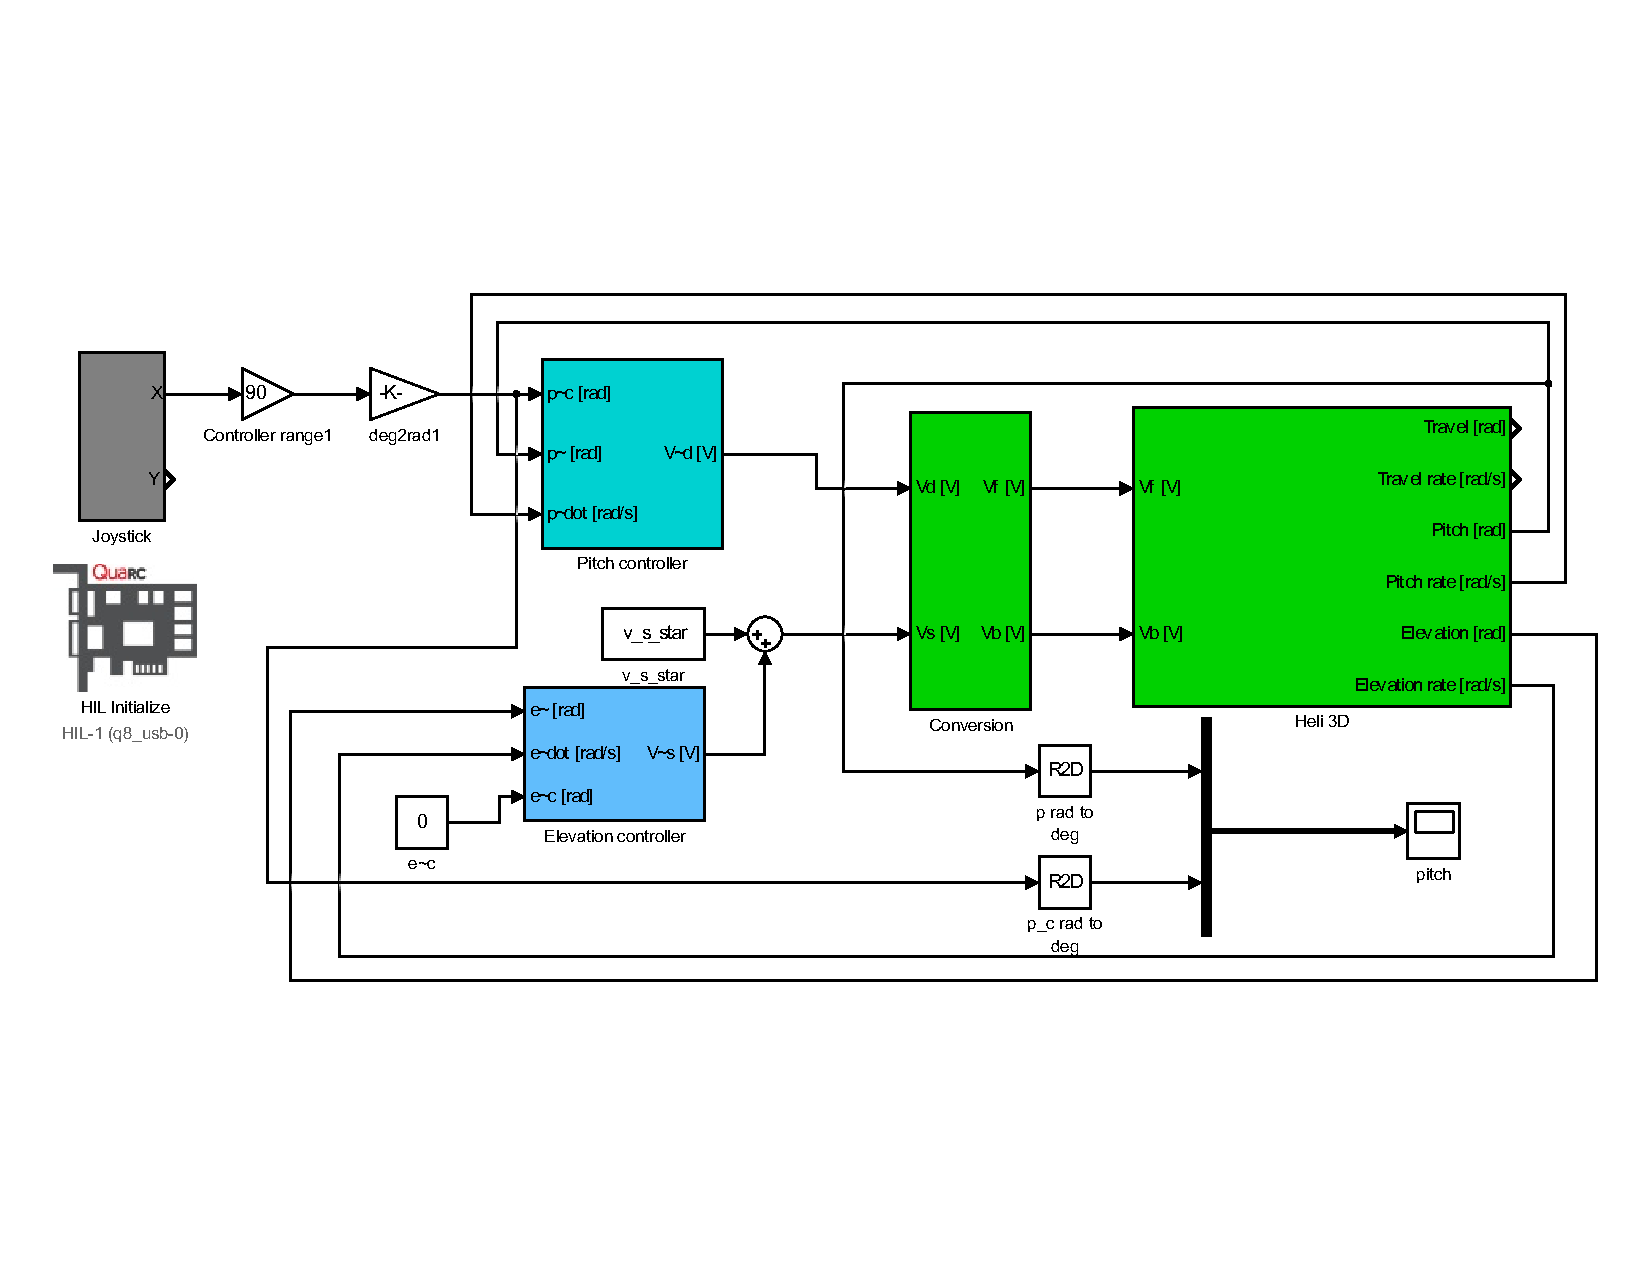
\includegraphics[trim=10 100 10 100, clip, width=\textwidth]{simulink/P2p1.pdf}
	\caption{Simulink implementation of system with pitch controller.}
\label{fig:monoPitch}
\end{figure}

\begin{figure}[!htb]
	\centering
	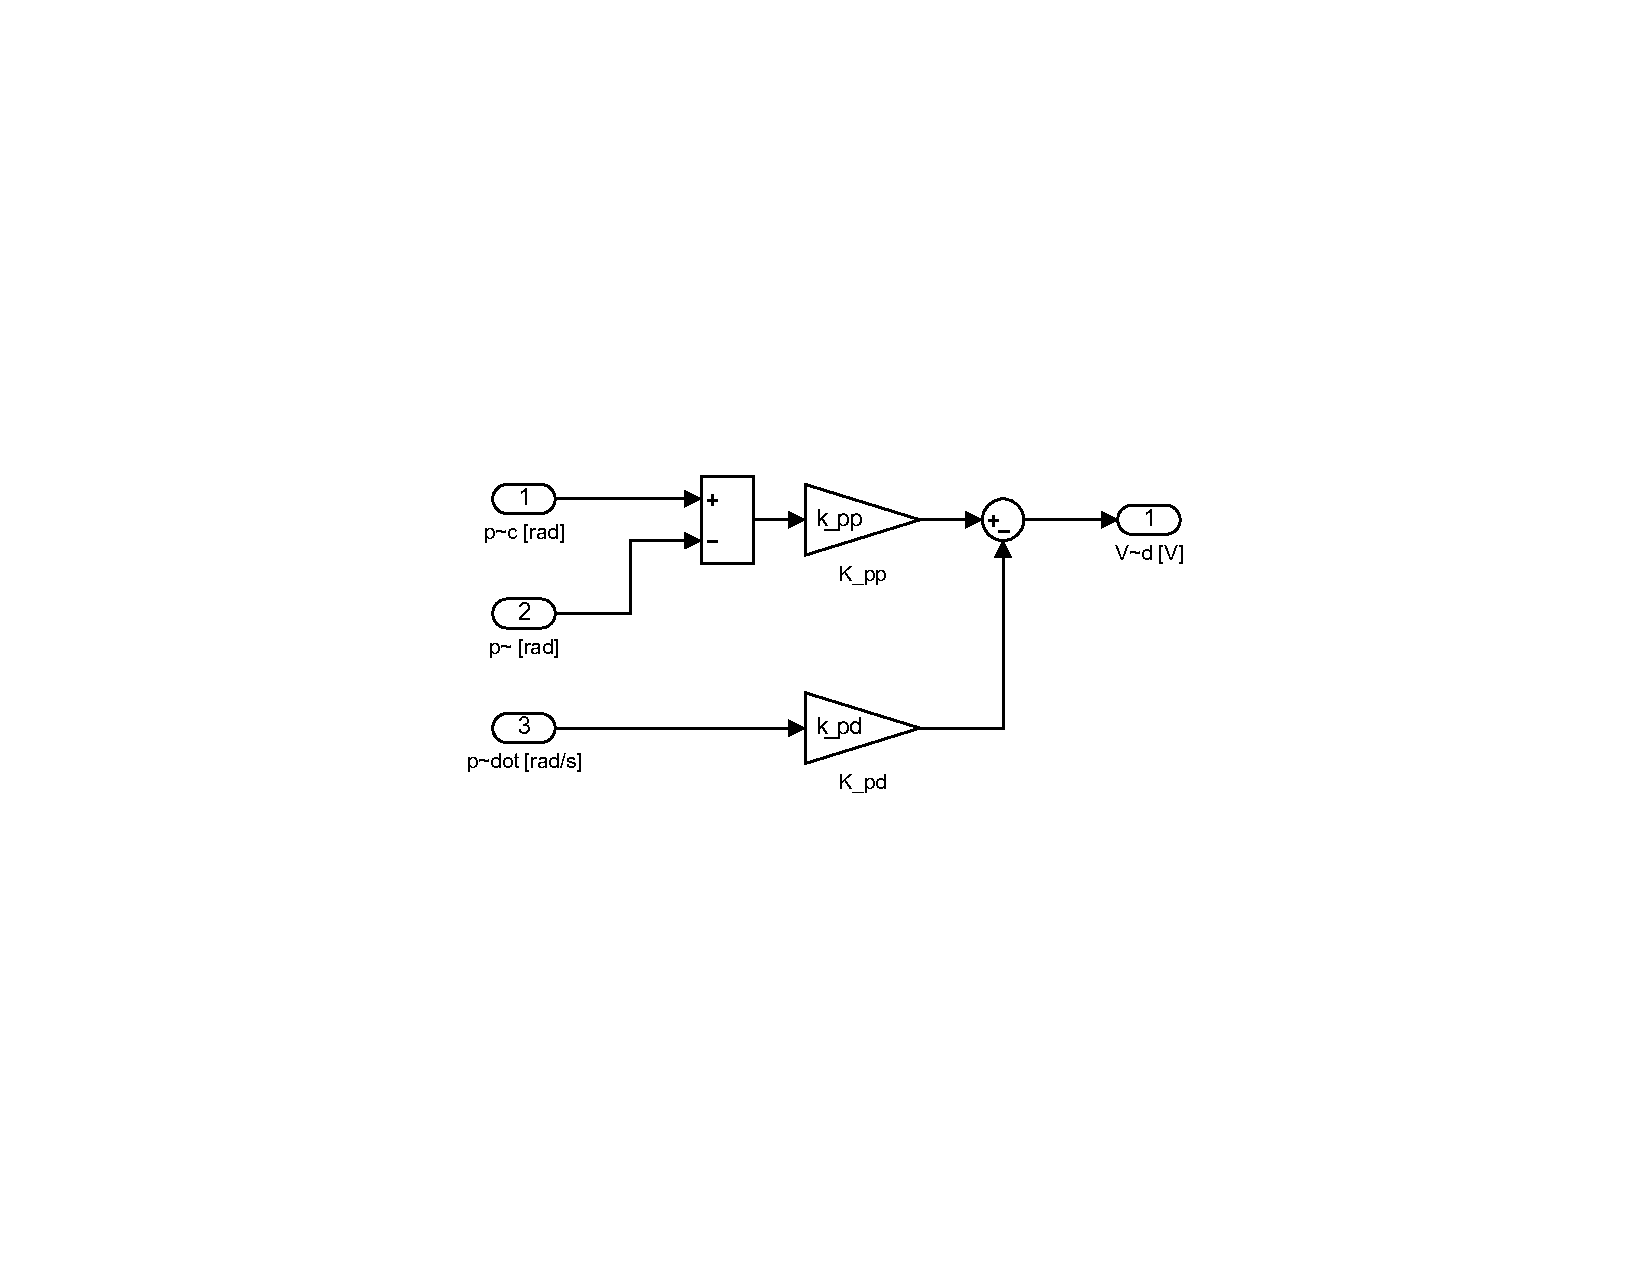
\includegraphics[trim=200 200 200 200,clip,width=\textwidth]{simulink/P2p1_pitch_reg.pdf}
	\caption{Simulink implementation of pitch controller.}
\label{fig:pitch_controller}
\end{figure}

\begin{figure}[!htb]
	\centering
	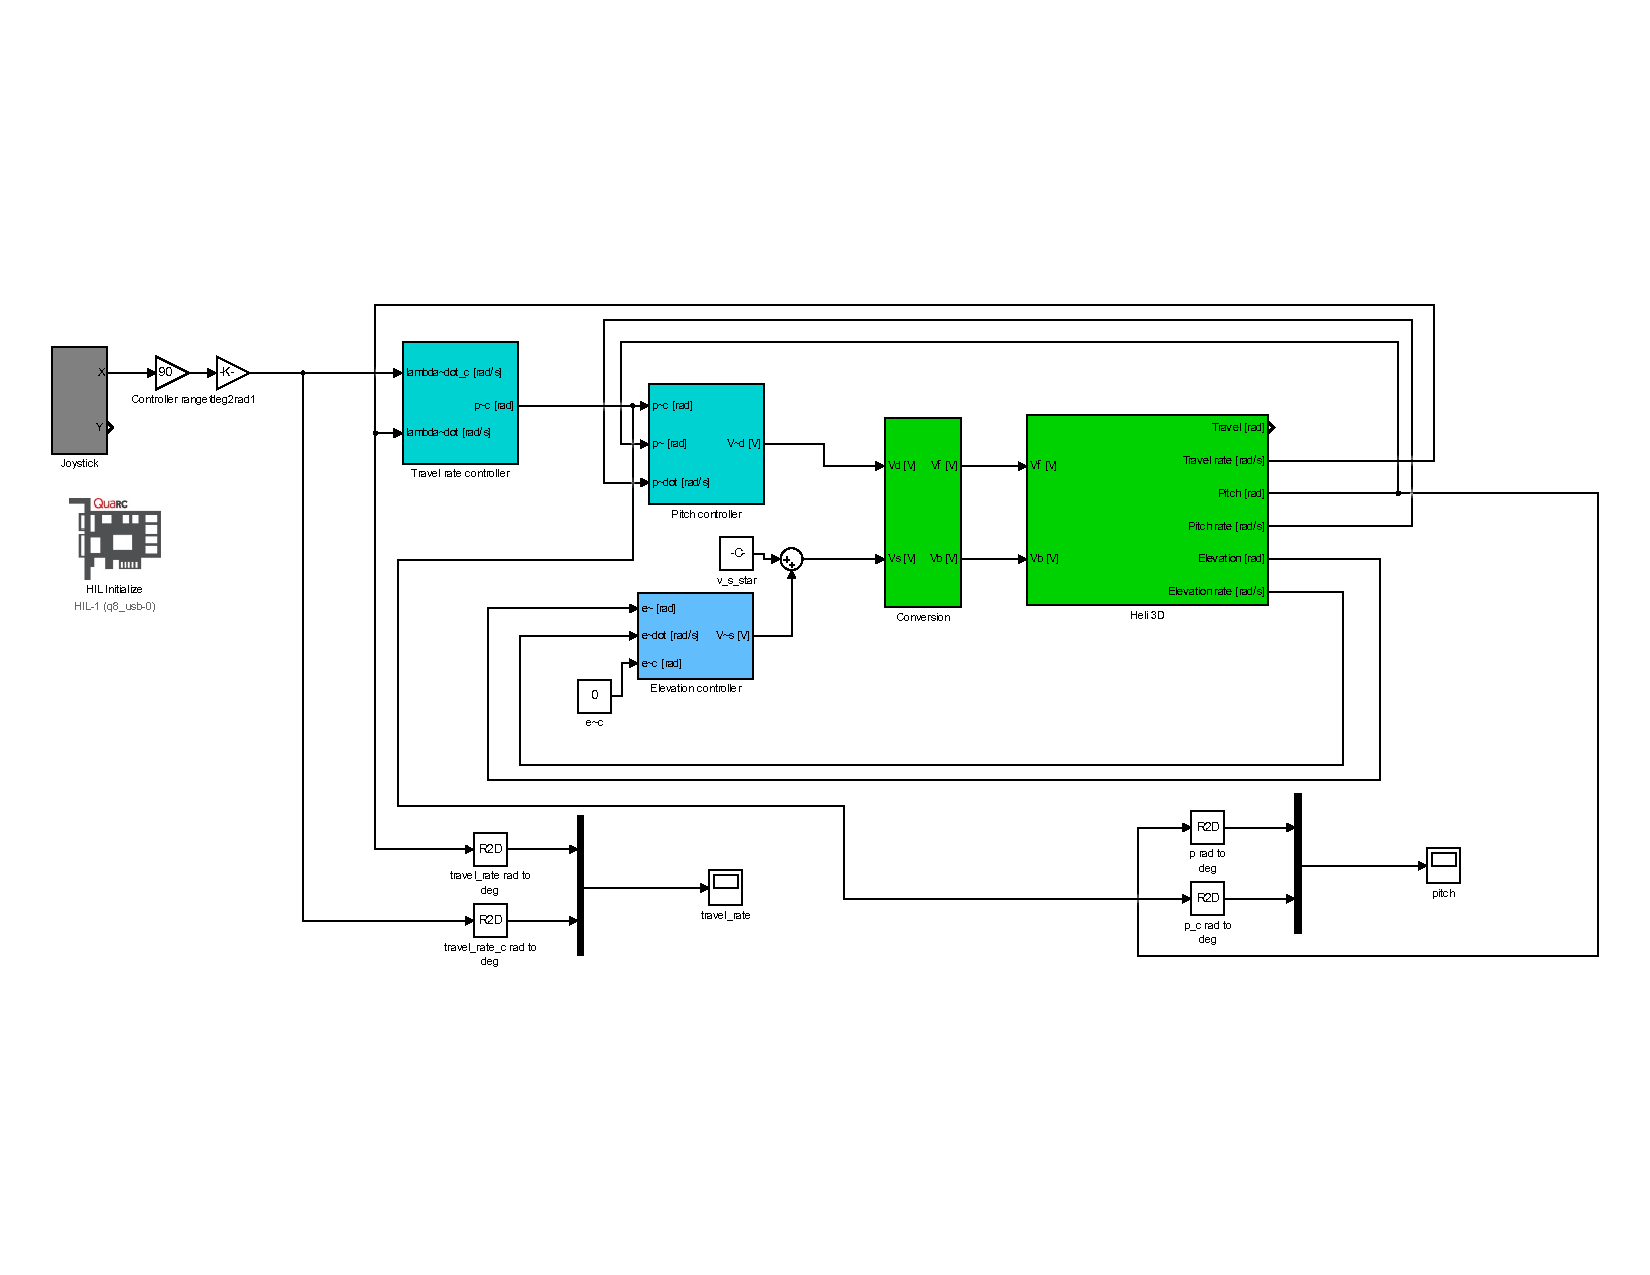
\includegraphics[trim=0 100 0 100, clip, width=\textwidth]{simulink/P2p2.pdf}
	\caption{Simulink implementation of system with travel rate controller and pitch controller.}
\label{fig:monoTravelPitch}
\end{figure}

\begin{figure}[!htb]
	\centering
	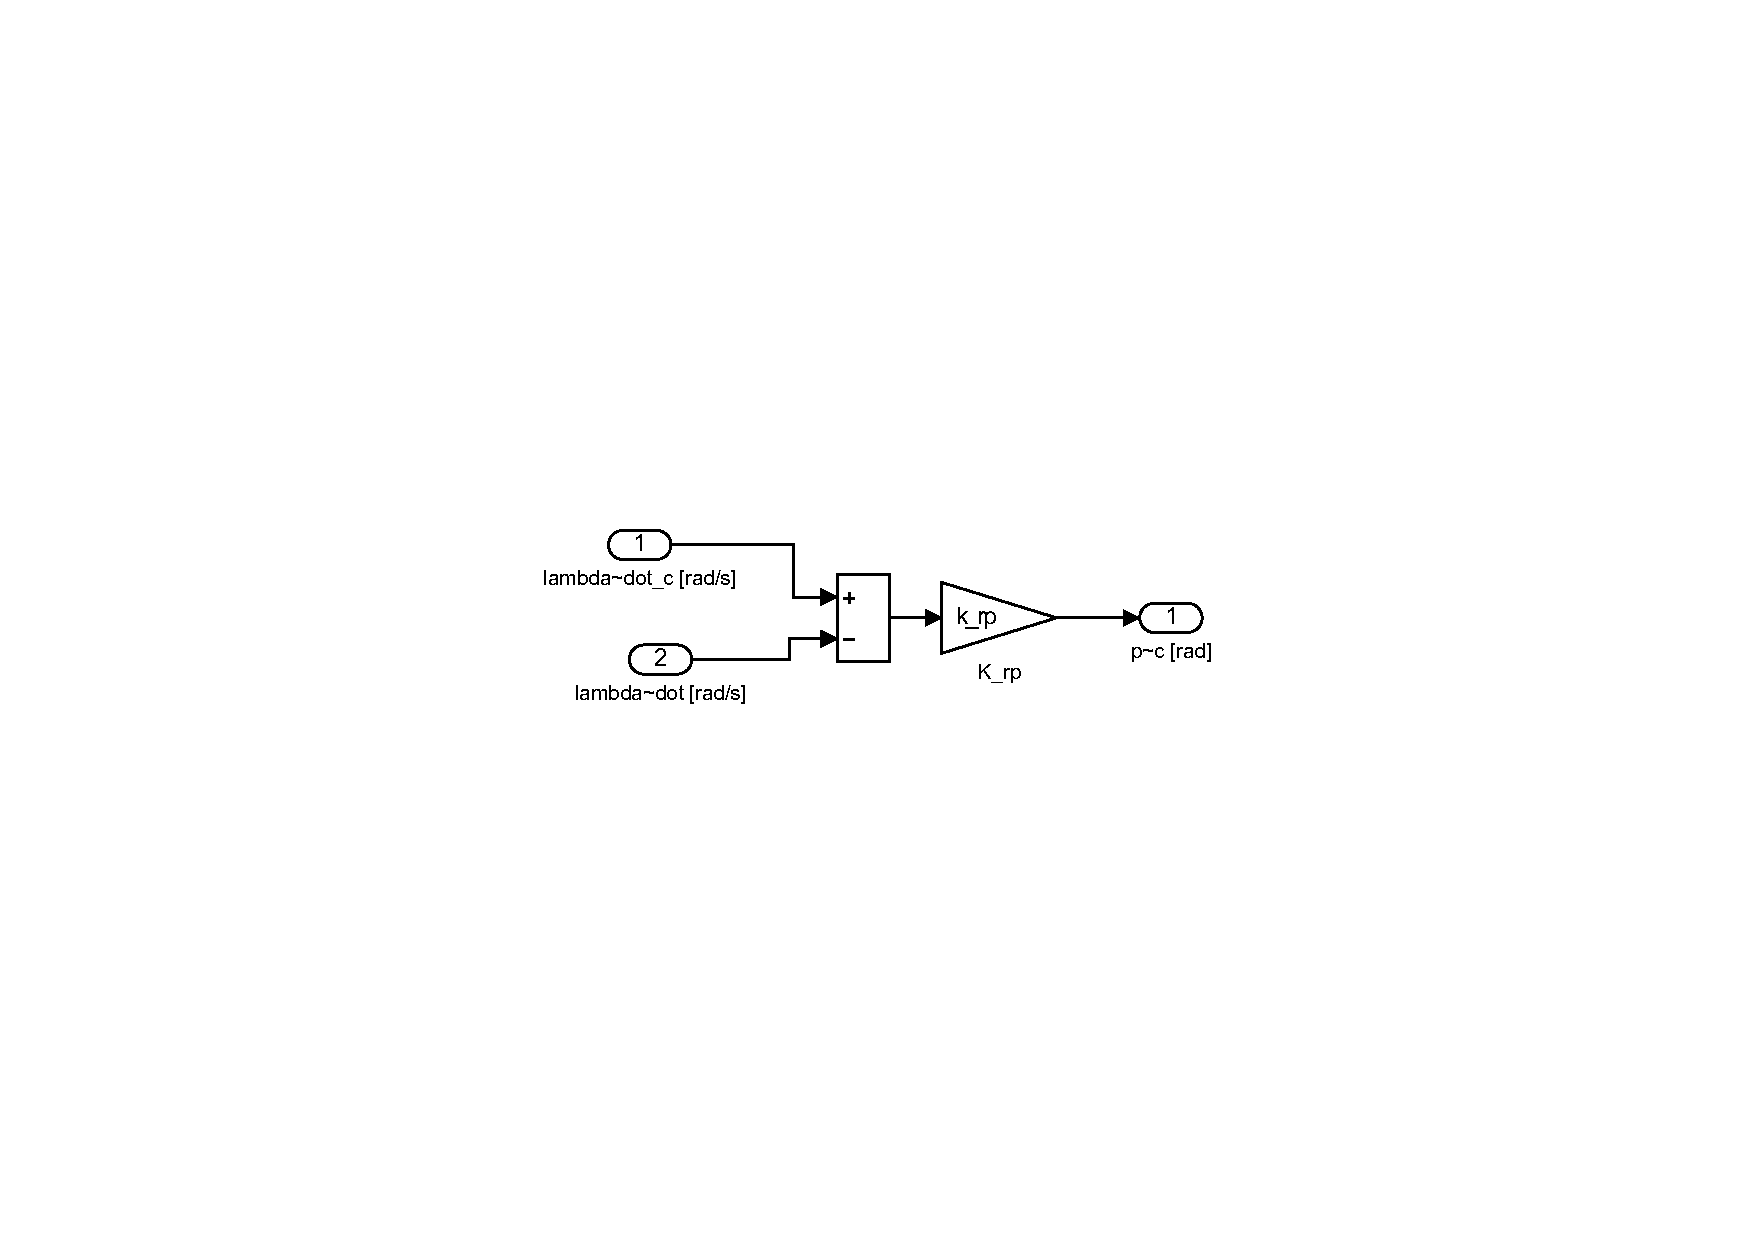
\includegraphics[trim=250 250 250 250, clip, width=\textwidth]{simulink/P2p2_travel_reg.pdf}
	\caption{Simulink implementation of travel rate controller}
\label{fig:monoTravel}
\end{figure}

\begin{figure}[!htb]
	\centering
	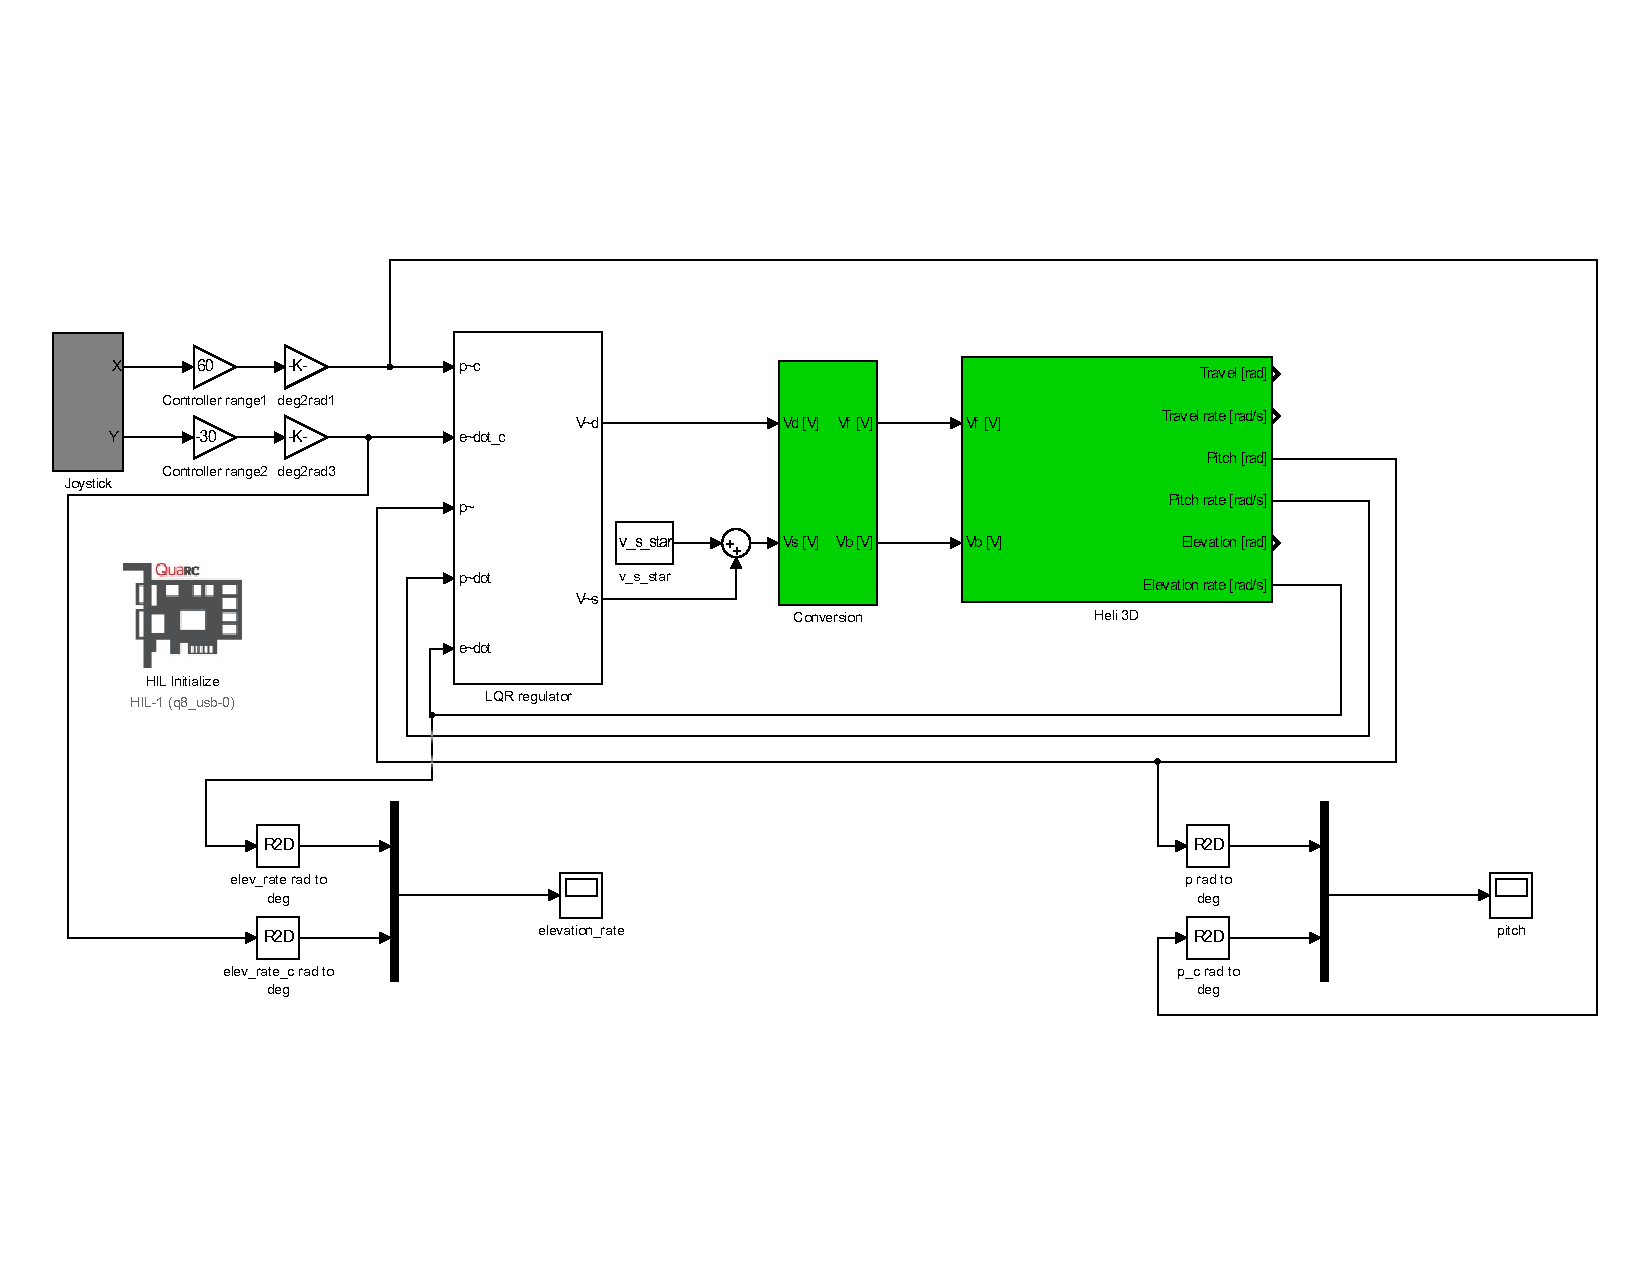
\includegraphics[trim=0 100 0 100, clip, width=\textwidth]{simulink/P3p2.pdf}
	\caption{Simulink implementation of system with LQR controller.}
\label{fig:LQRSystem}
\end{figure}

\begin{figure}[!htb]
	\centering
	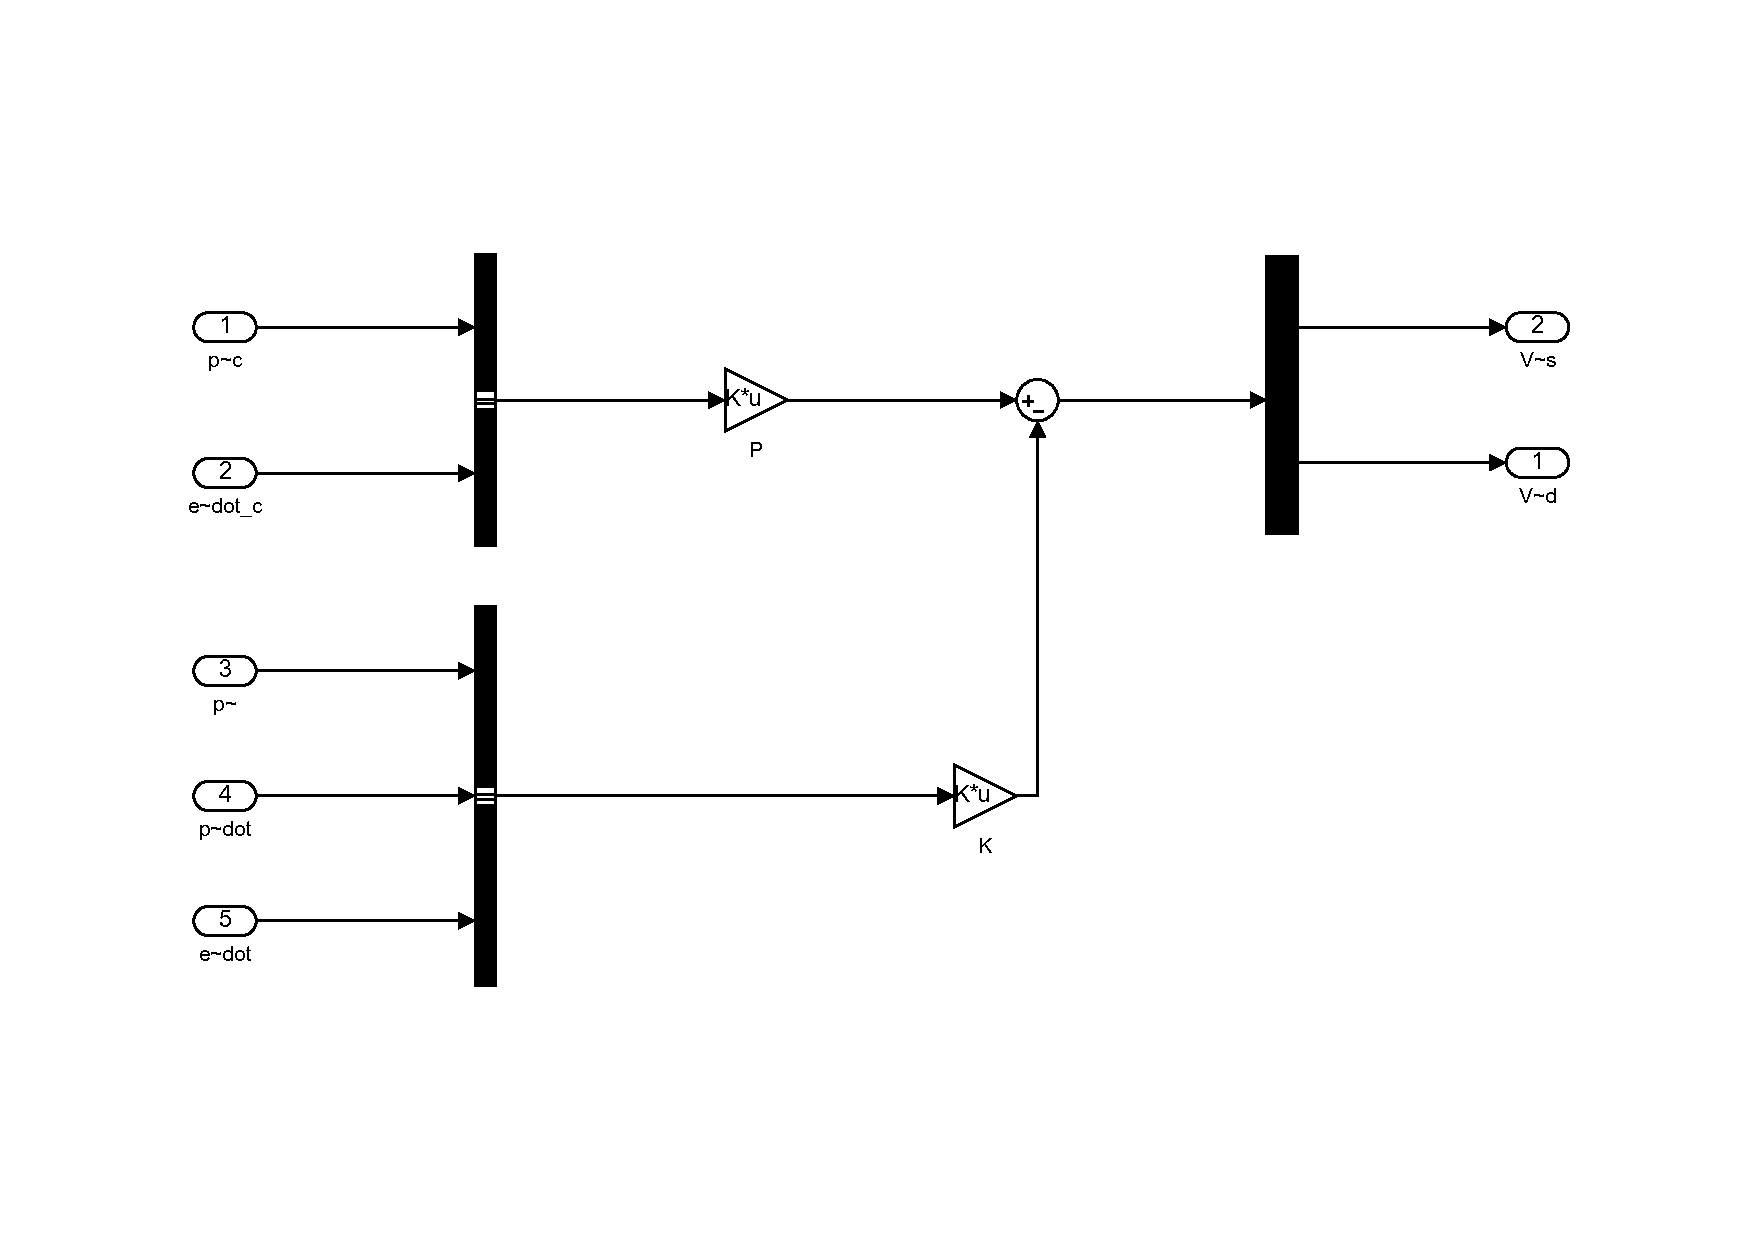
\includegraphics[trim=0 100 0 125, clip, width=\textwidth]{simulink/P3p2_LQR_reg.pdf}
	\caption{Simulink implementation of LQR controller.}
\label{fig:LQR}
\end{figure}

\begin{figure}[!htb]
	\centering
	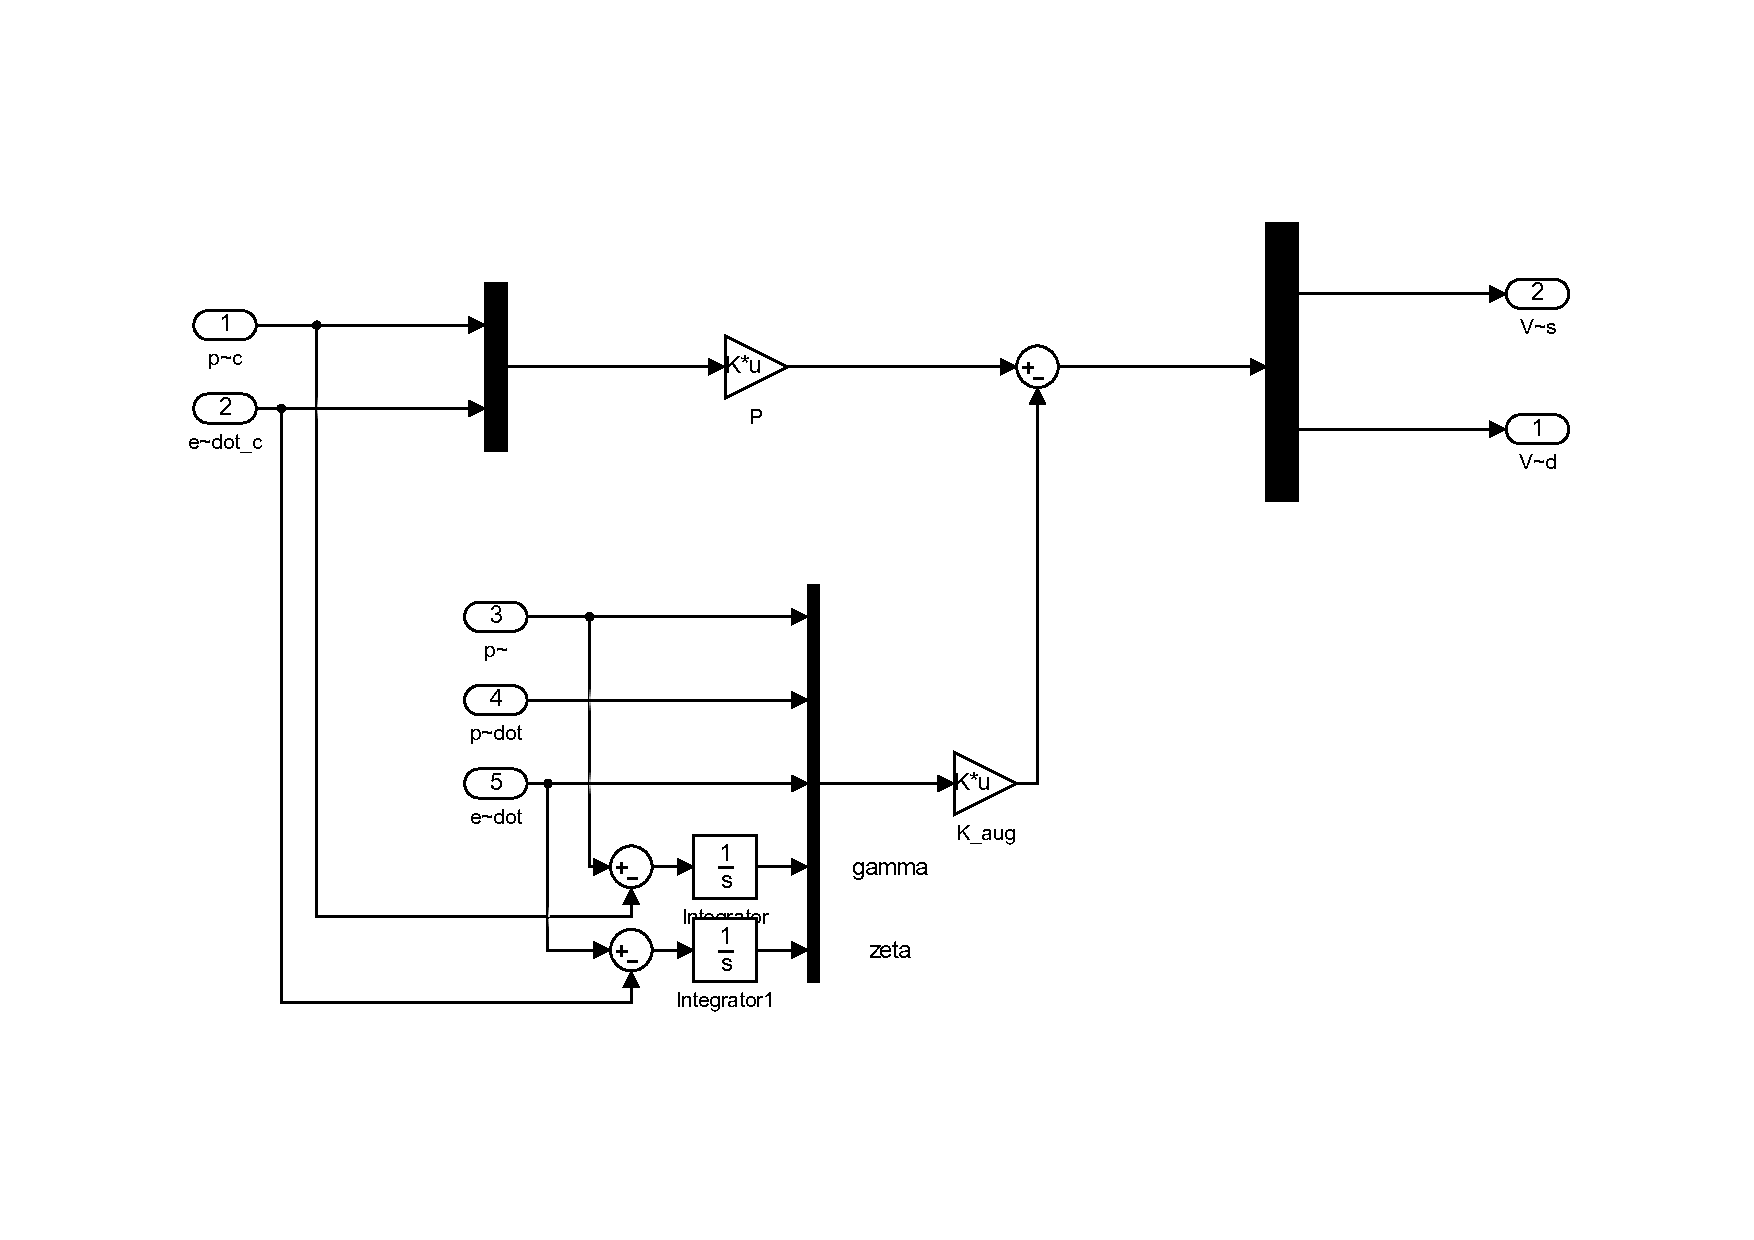
\includegraphics[trim=0 100 0 100, clip, width=\textwidth]{simulink/P3p3_LQR_reg_integral.pdf}
	\caption{Simulink implementation of LQR controller with added integral effect.}
\label{fig:LQRIntegral}
\end{figure}

\begin{figure}[!htb]
	\centering
	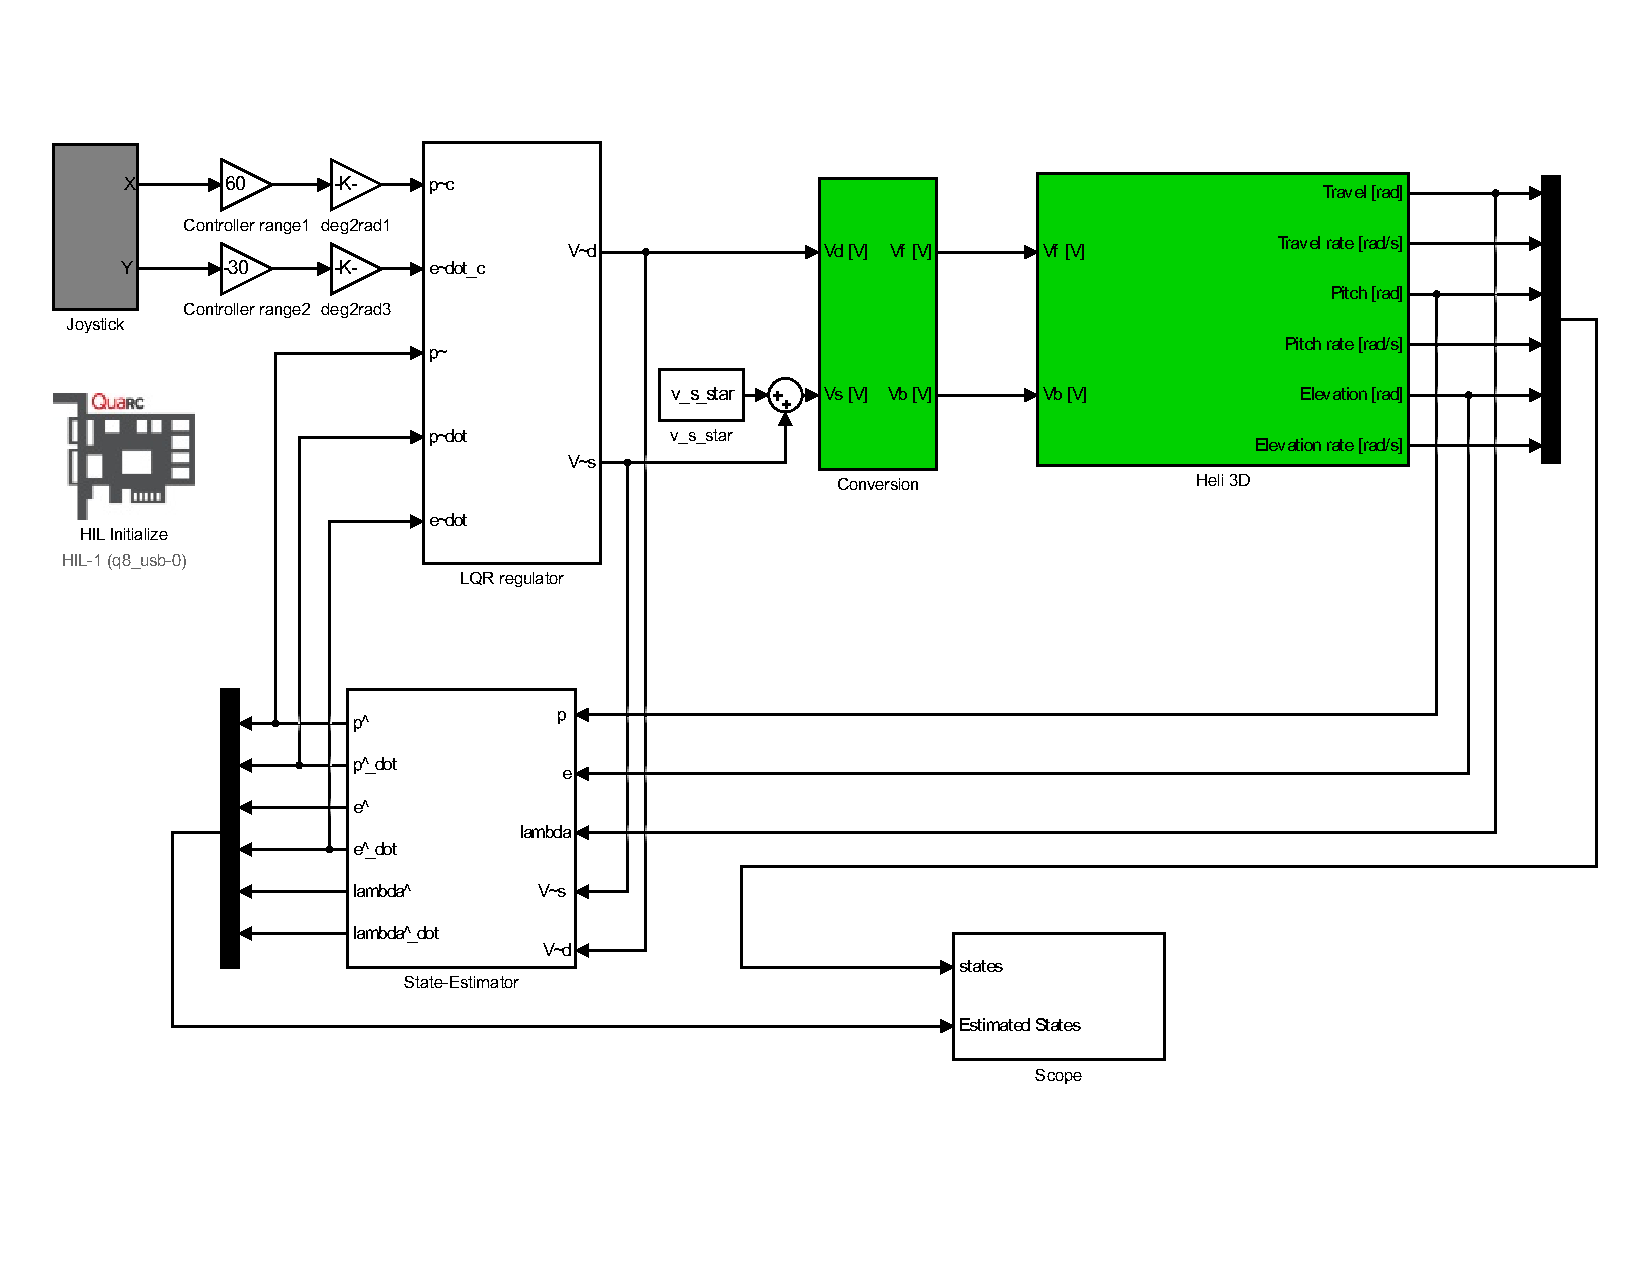
\includegraphics[trim=0 100 0 50, clip, width=\textwidth]{simulink/P4p2.pdf}
	\caption{Simulink implementation of system with observer.}
\label{fig:ObserverSystem}
\end{figure}

\begin{figure}[!htb]
	\centering
	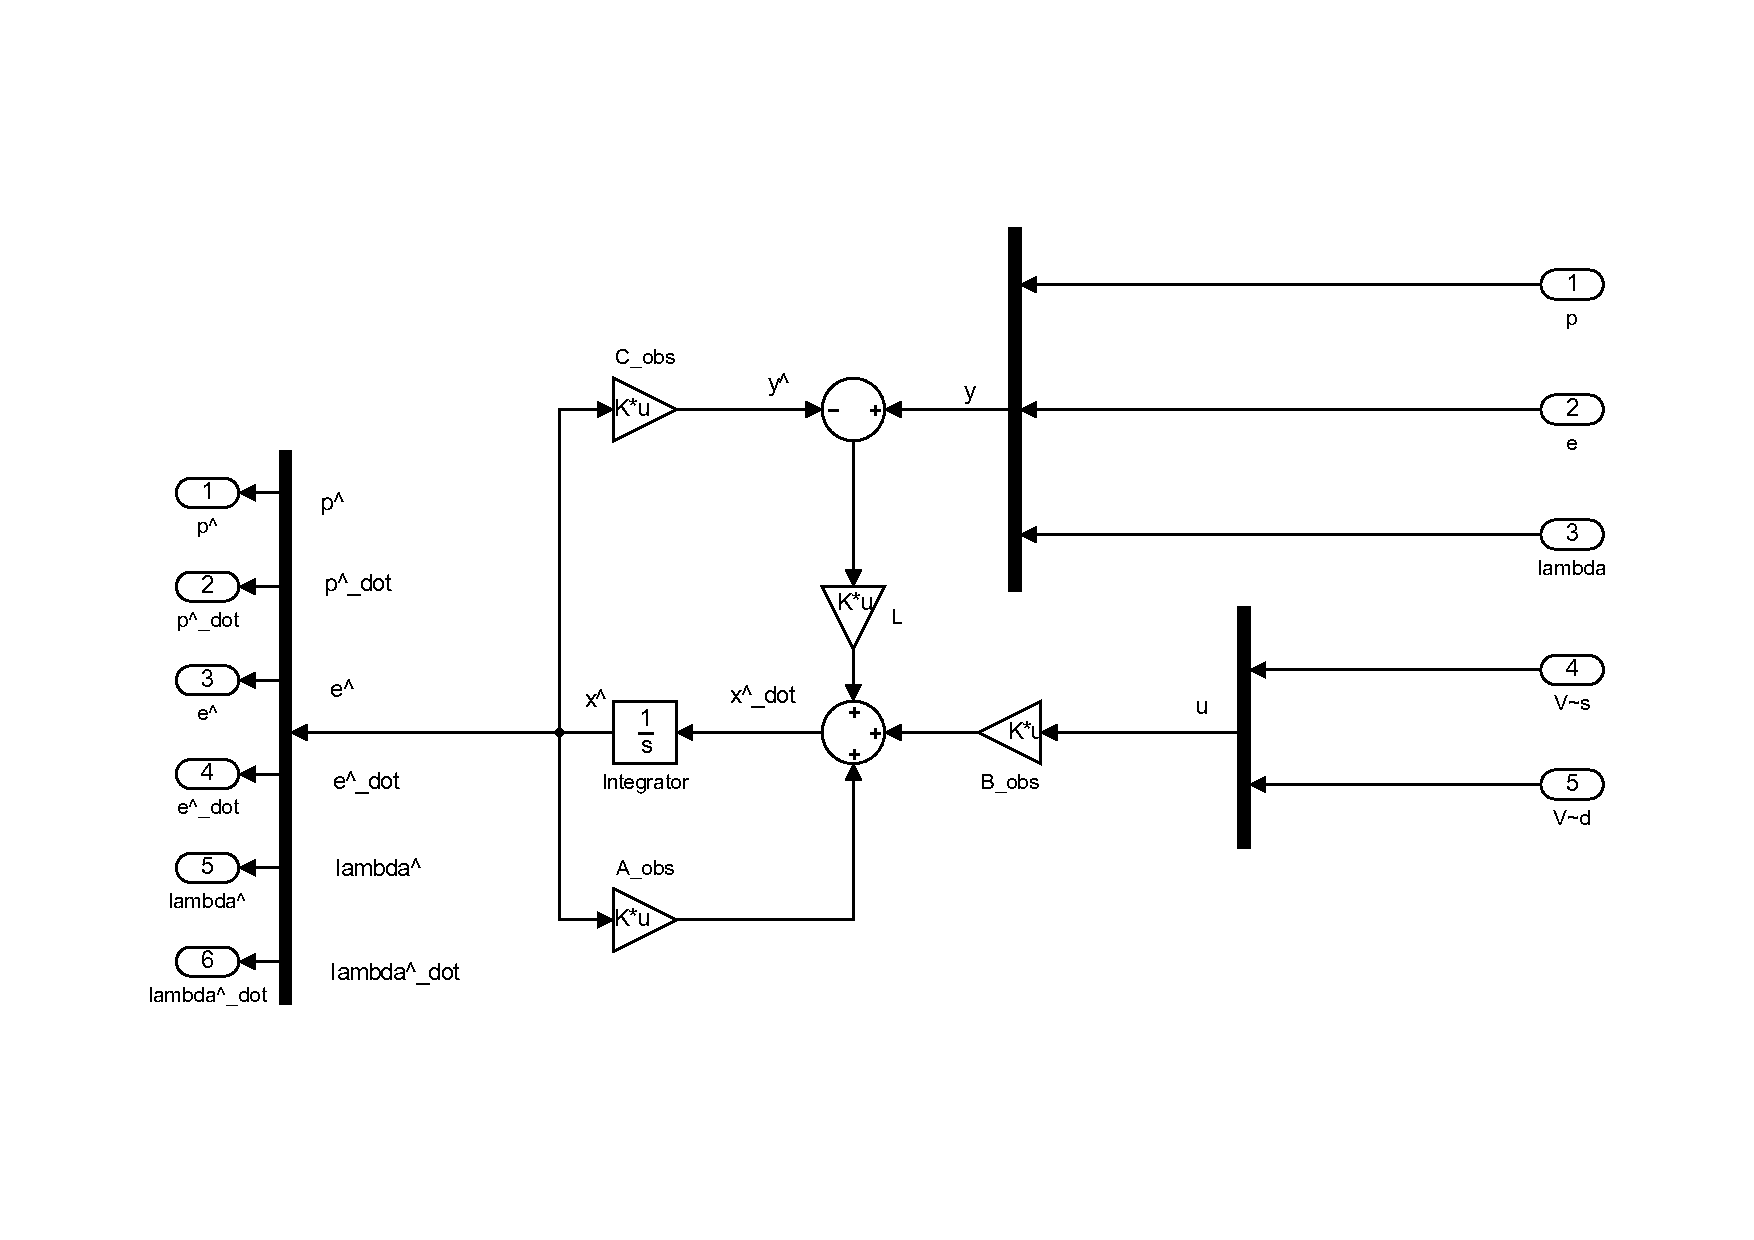
\includegraphics[trim=0 100 0 100, clip, width=\textwidth]{simulink/P4p2_state_estimator.pdf}
	\caption{Simulink implementation of observer.}
\label{fig:Observer}
\end{figure}

\clearpage
\section{Plots}

\begin{figure}[!htb]
	\centering
	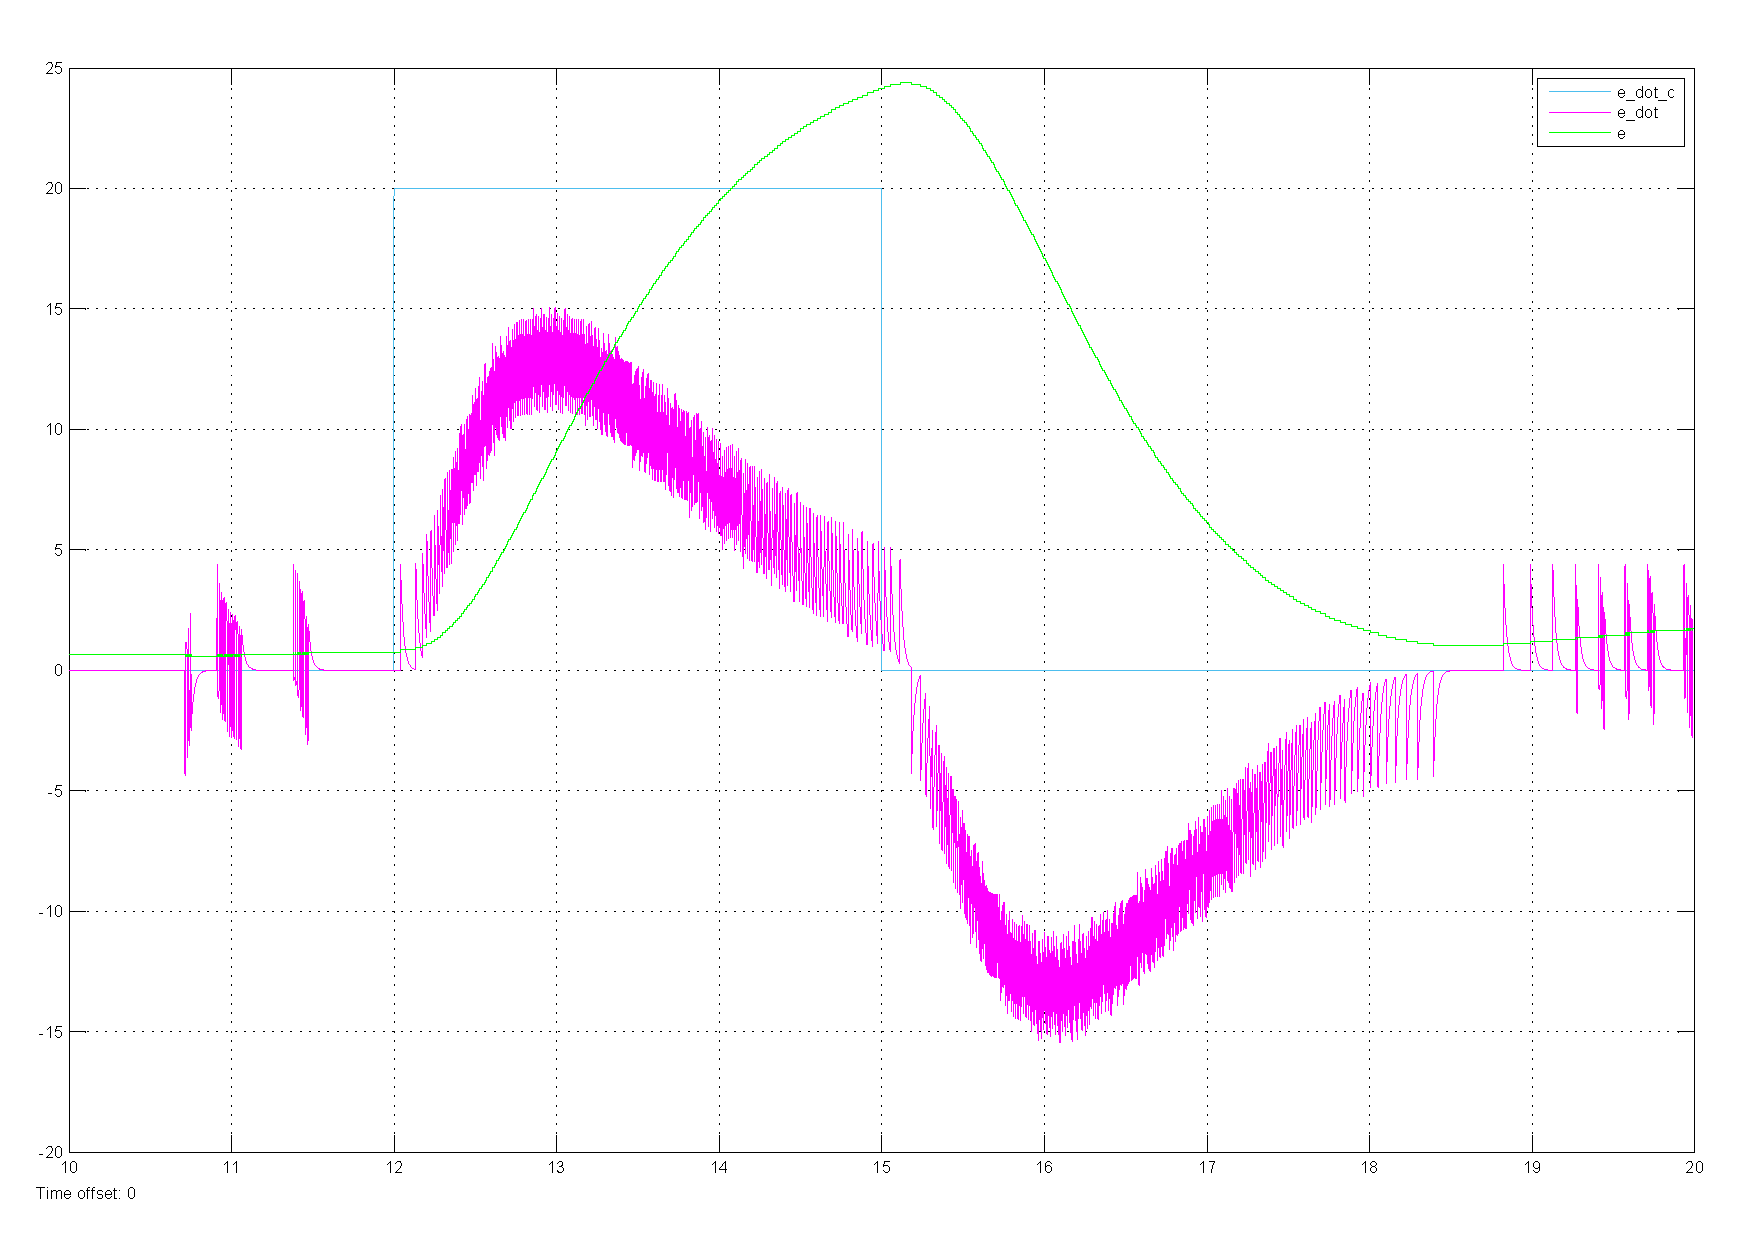
\includegraphics[width=\textwidth]{plots/P3p2_LQR_without_integral_elevation.pdf}
	\caption{Elevation response for LQR without integral effect.}
\label{fig:P3p2ElevWithoutIntegral}
\end{figure}

\begin{figure}[!htb]
	\centering
	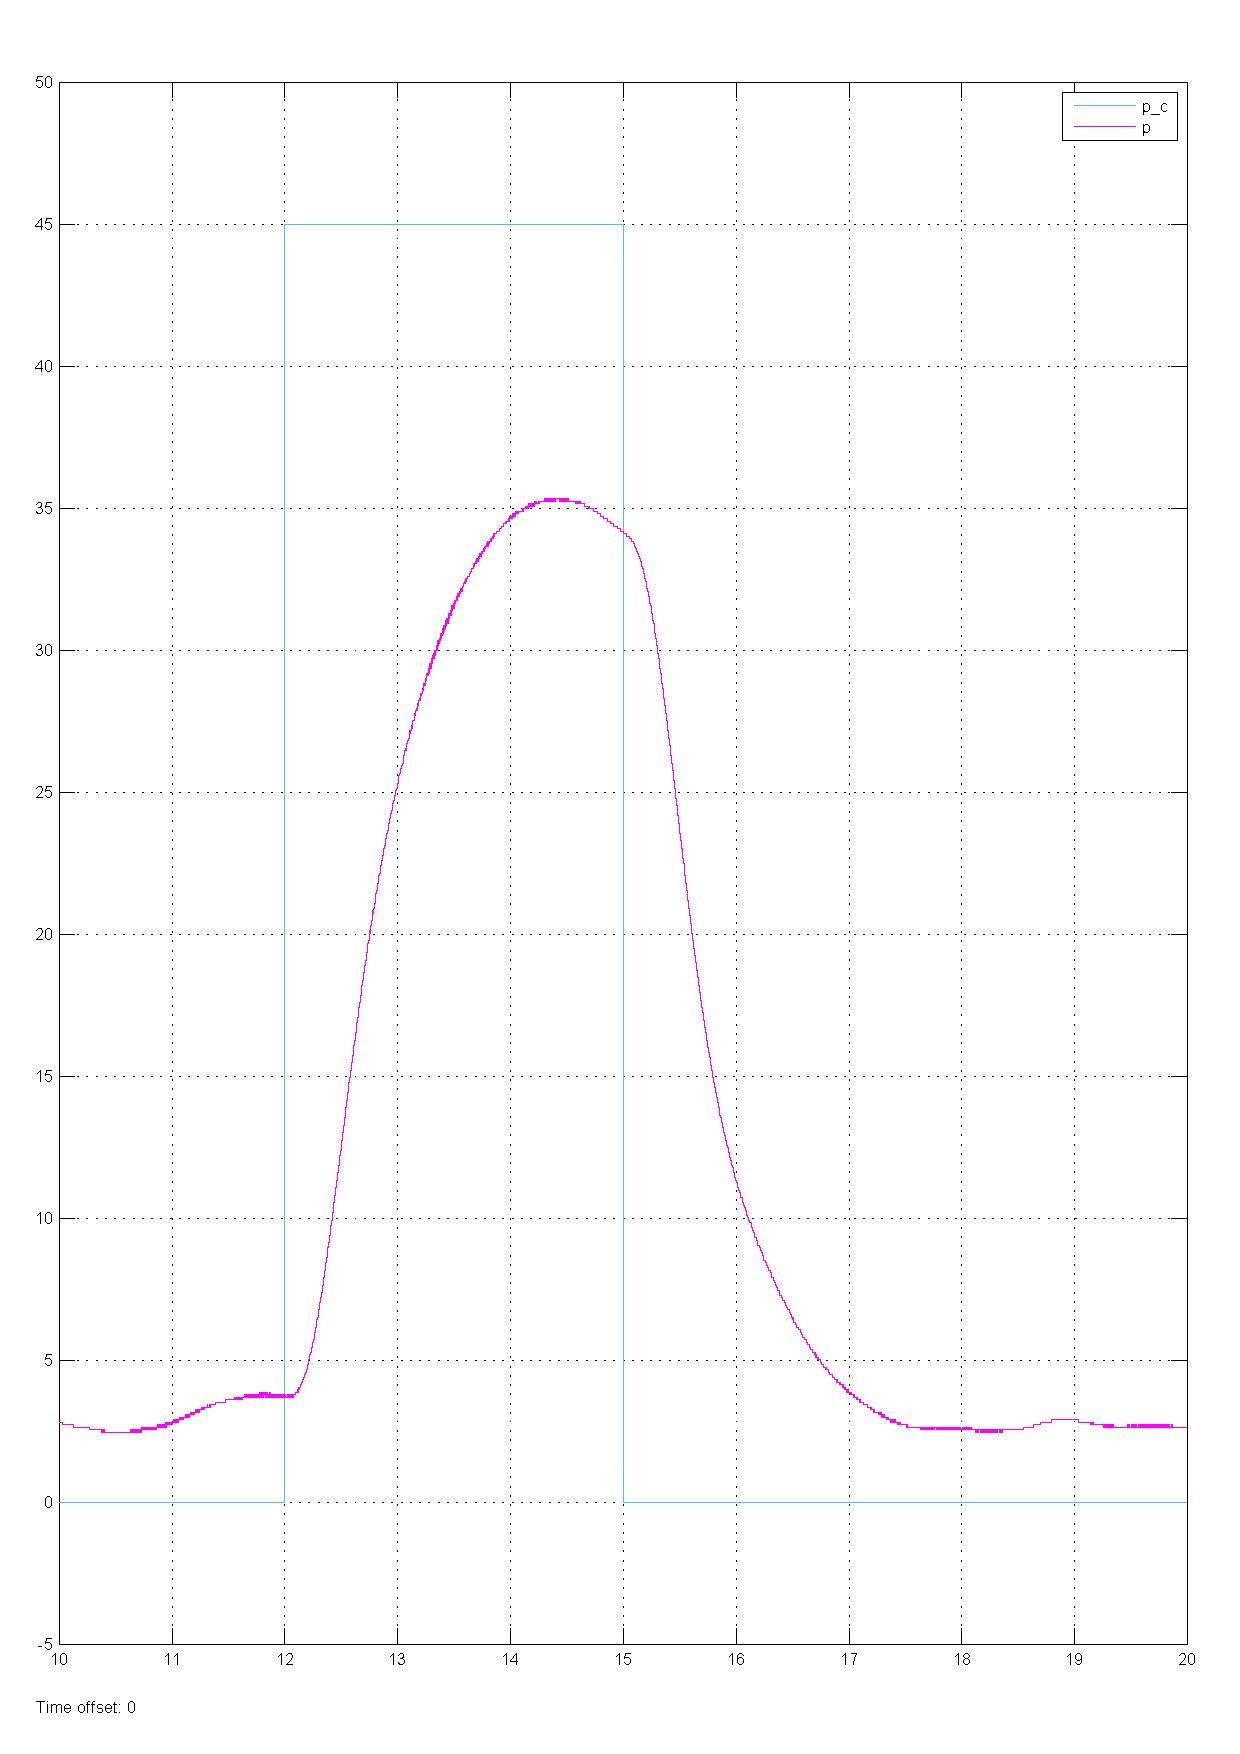
\includegraphics[width=\textwidth]{plots/P3p2_LQR_without_integral_pitch.pdf}
	\caption{Pitch response for LQR without integral effect.}
\label{fig:P3p2PitchWithoutIntegral}
\end{figure}

\begin{figure}[!htb]
	\centering
	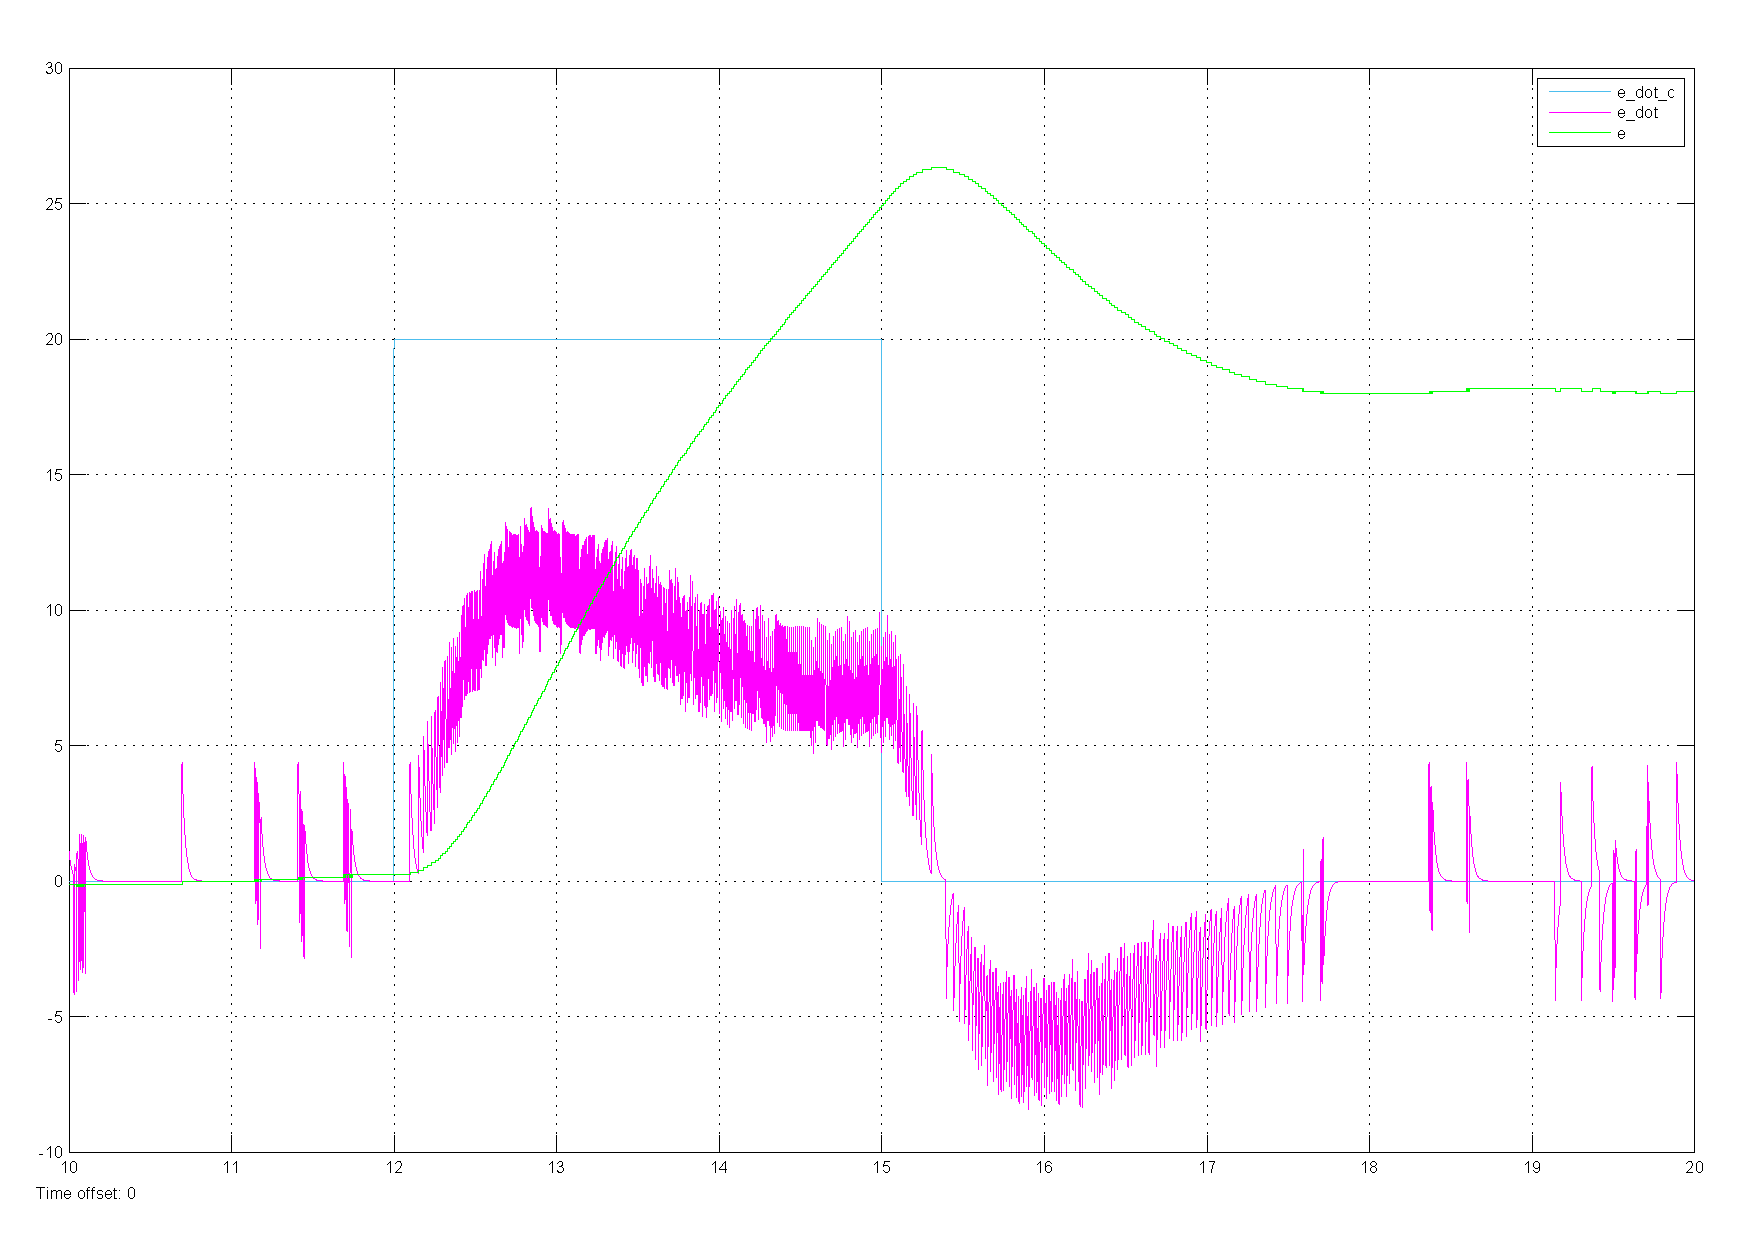
\includegraphics[width=\textwidth]{plots/P3p3_LQR_with_integral_elevation.pdf}
	\caption{Elevation response for LQR with integral effect.}
\label{fig:P3p3ElevWithIntegral}
\end{figure}

\begin{figure}[!htb]
	\centering
	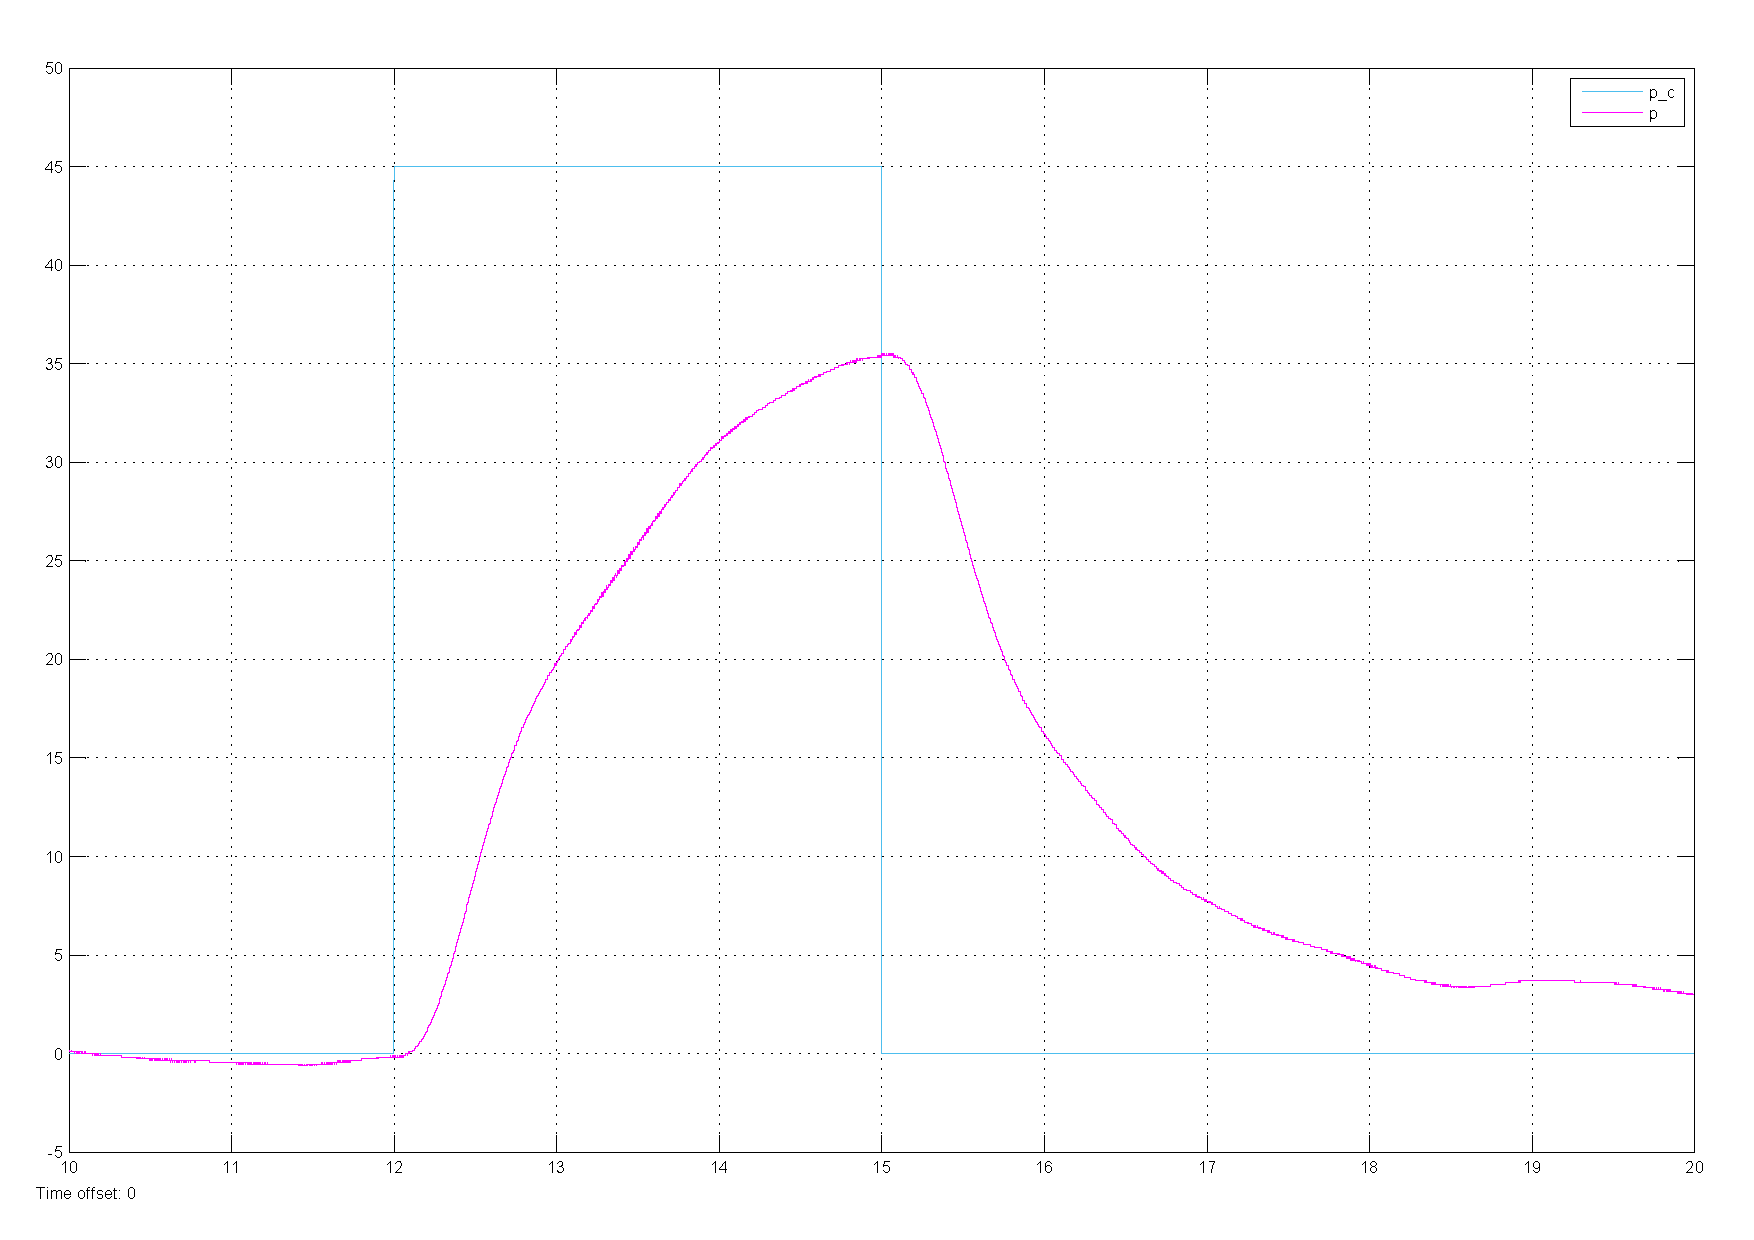
\includegraphics[width=\textwidth]{plots/P3p3_LQR_with_integral_pitch.pdf}
	\caption{Pitch response for LQR with integral effect.}
\label{fig:P3p2PitchWithIntegral}
\end{figure}

\begin{figure}[!htb]
	\centering
	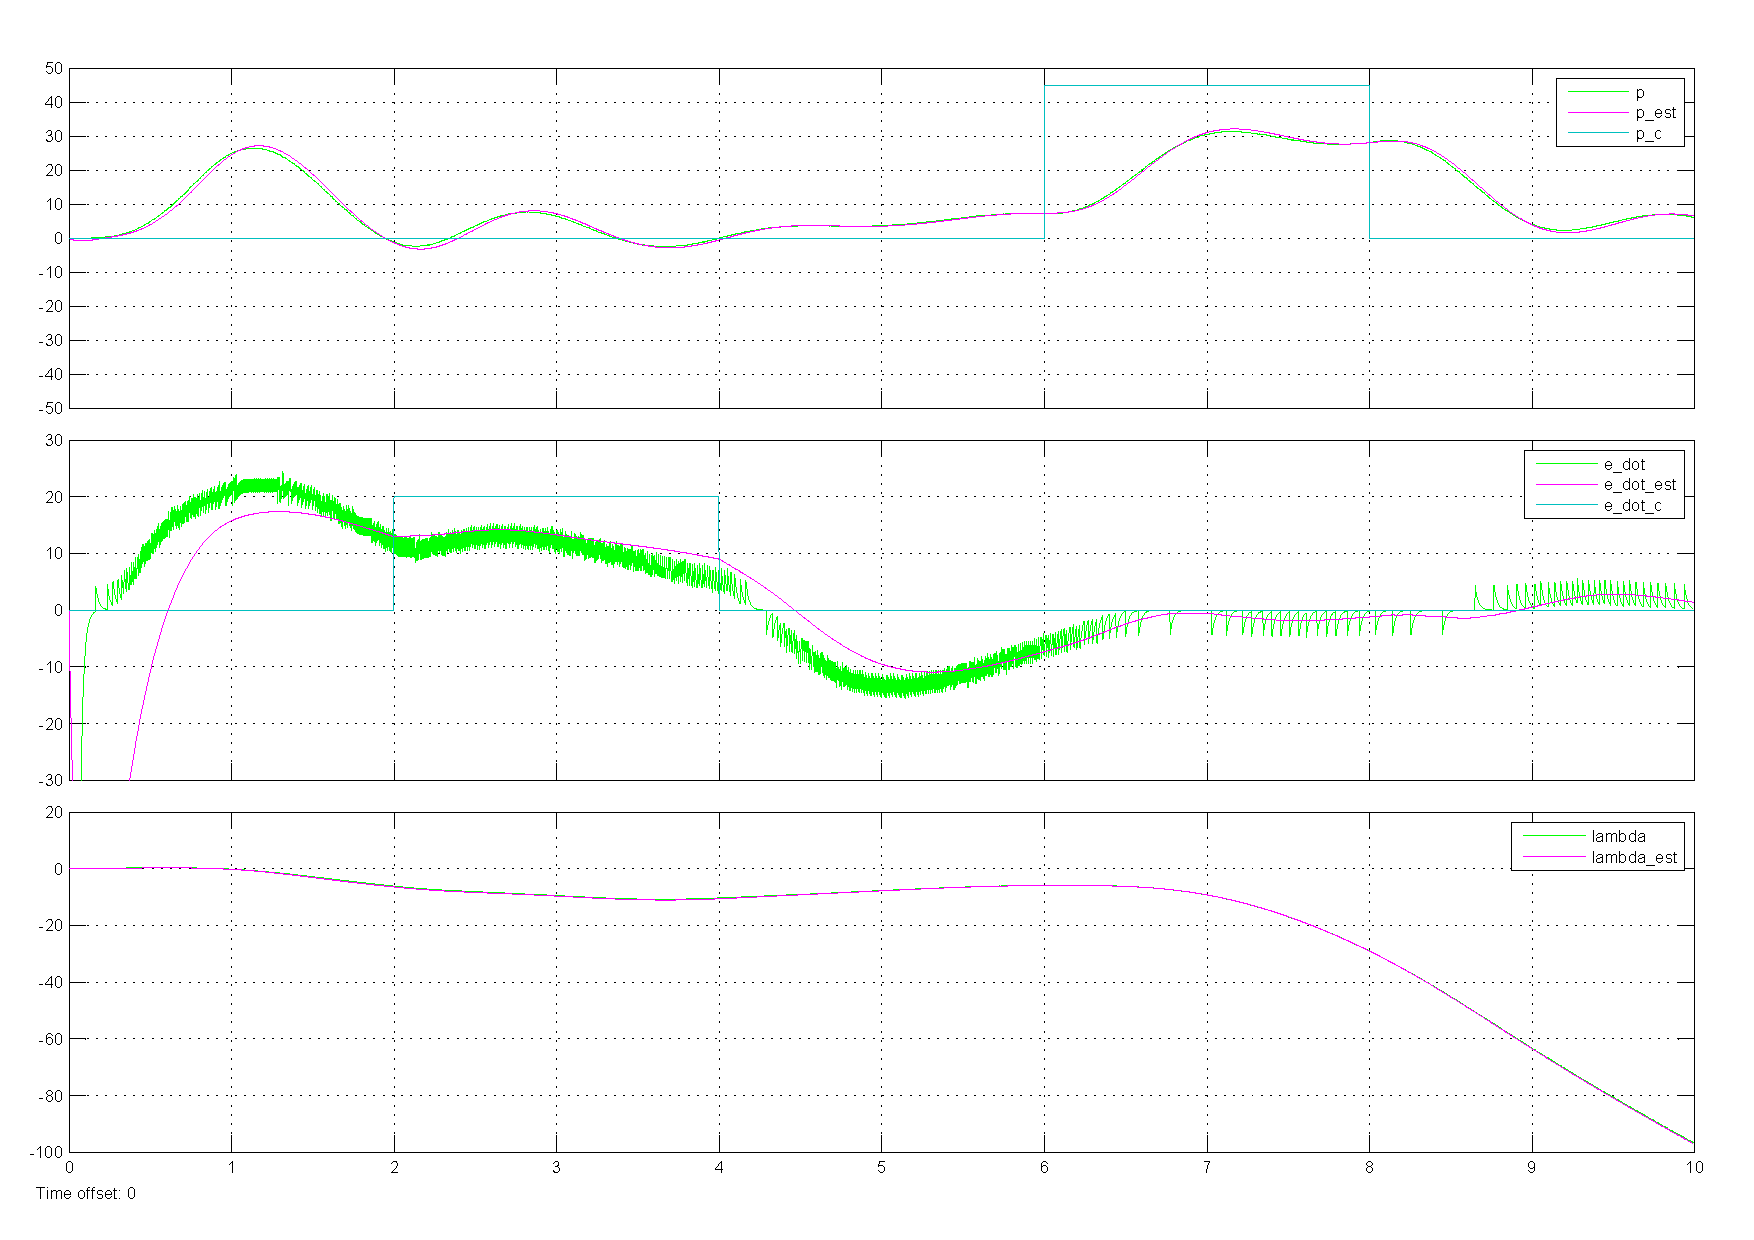
\includegraphics[width=\textwidth]{plots/P4p2_EST_without_integral.pdf}
	\caption{Full state observer with LQR controller without integral effect.}
\label{fig:ESTWithoutIntegral}
\end{figure}

\begin{figure}[!htb]
	\centering
	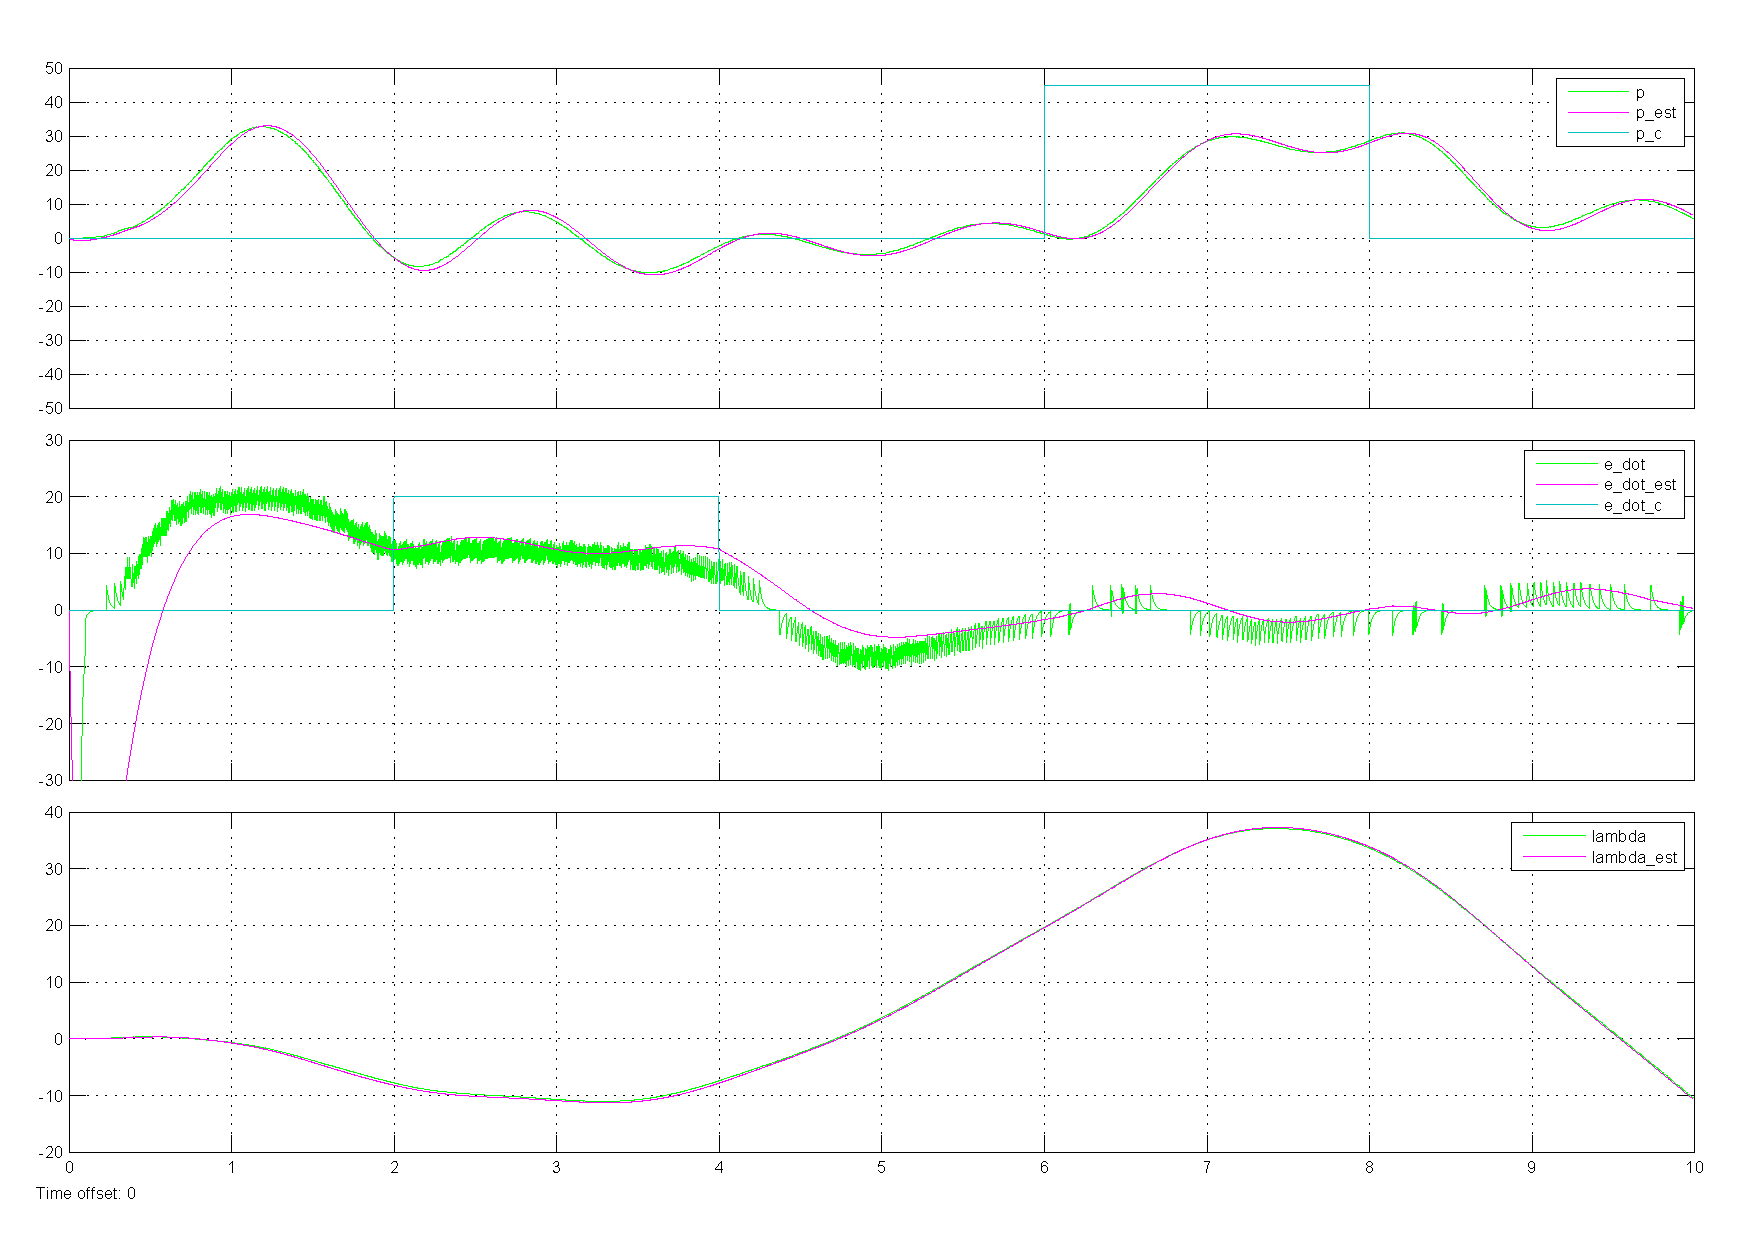
\includegraphics[width=\textwidth]{plots/P4p2_EST_with_integral.pdf}
	\caption{Full state observer with LQR controller with integral effect.}
\label{fig:ESTWithIntegral}
\end{figure}

\begin{figure}[!htb]
	\centering
	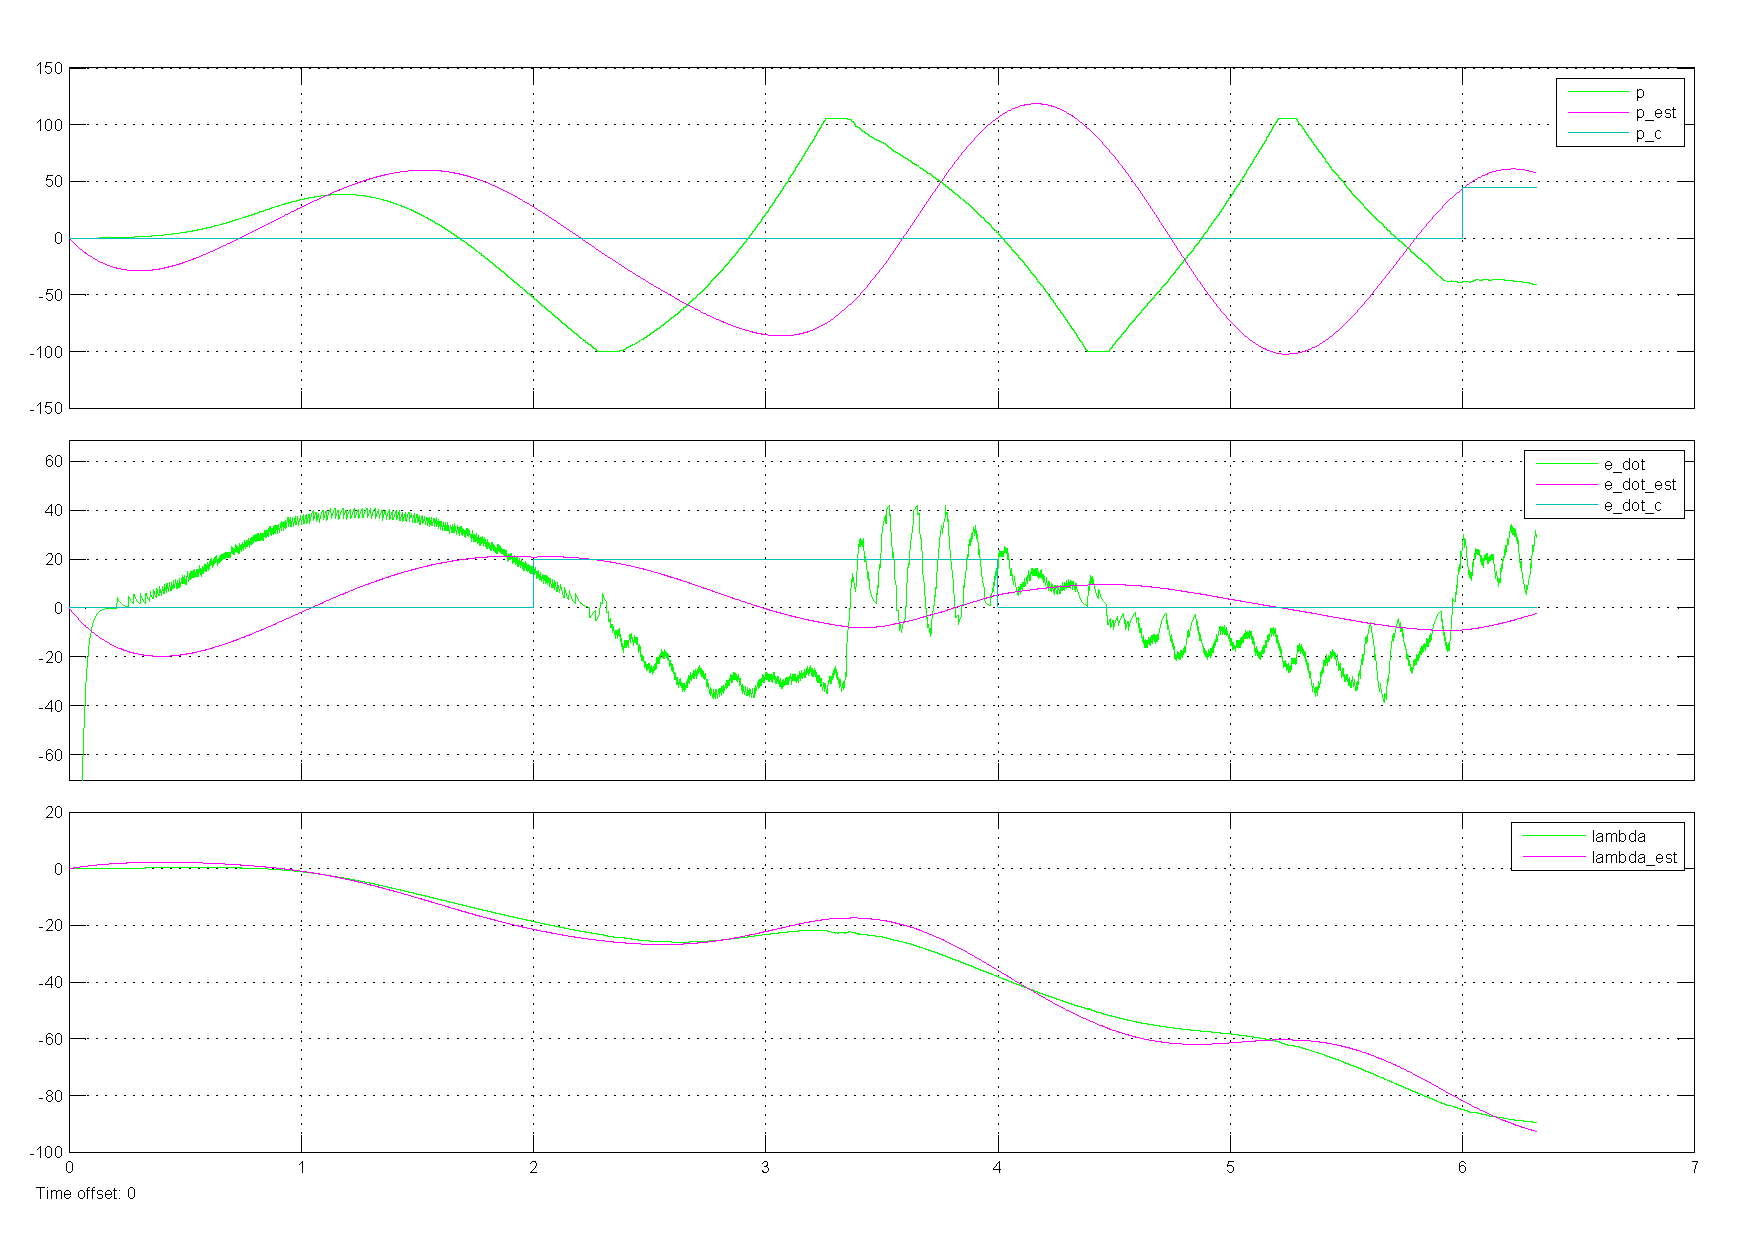
\includegraphics[width=\textwidth]{plots/P4p3_EST_not_p.pdf}
	\caption{Minimal state observer with LQR controller with integral effect.}
\label{fig:ESTnotp}
\end{figure}